\documentclass[a4paper, 12pt, oneside, openany, final, pdftex]{book}

%%%%%%%%%%%%%%%%%%%%%%%%%%%%%%%%%%%%%%%%%%%%%%%%%%%%%%%%%%%%%%%%%%%%%%%%%%%%%%%%
% PAKETI
%%%%%%%%%%%%%%%%%%%%%%%%%%%%%%%%%%%%%%%%%%%%%%%%%%%%%%%%%%%%%%%%%%%%%%%%%%%%%%%%

% geometrija stranice
% margine postavljene kao sto i pise u obrascu DR.SC.08
\usepackage[margin=25mm,centering]{geometry} 

% prihvaca tex kod kao UTF-8 omogućavajući
% pisanje znakova s dijakriticima unutar datoteke
% npr. možemo pisati 'č' umjesto č
% PAZITI DA SU DATOTEKE STVARNO SPREMLJENE KAO UTF-8
% nije korisno ako se namjerava koristiti 'latexdiff'
\usepackage[utf8]{inputenc}
% korisnici Windowsa trebaju odkomentirati
% sljedeću liniju te zakomentirati prijašnju
% \usepackage[utf-8]{inputenc}

% omogućiti ispisivanje naših znakova u dokumentu 
\usepackage[T1]{fontenc}

% koristi novu verziju fonta (Latin Modern)
\usepackage{lmodern}

% Palatino font (blizu Arial-a)
%\usepackage[sc]{mathpazo}

% Times New Roman
%\usepackage{mathptmx}
% ili
%\usepackage{txfonts}

% koristan paket kad stvaranja pdf-a
\usepackage[activate={true,nocompatibility},
	final,
	tracking=true,
	kerning=true,
	spacing=true,
	factor=1100,
	stretch=10,
	shrink=10]{microtype}
\microtypecontext{spacing=nonfrench}
%\usepackage{microtype}

% babel !
\usepackage[croatian, english]{babel}
\usepackage{csquotes}

% captioni ce biti centrirani te će im ime
% biti podebljano. Poslije imena tablica (npr. Tablica 1.1:)
% slijedi nova linija. Nakon tablica slijedi mala praznina
\usepackage[center,labelfont=bf]{caption}
	\captionsetup[table]{skip=10pt, labelsep=newline}

% koristan paket za pisanje url-ova u tekstu
\usepackage{url}

% paketi za oblikovanje tablica
\usepackage{booktabs}
\usepackage{multirow}
\usepackage{array}
\newcolumntype{t}{>{\ttfamily}c}

% paketi za oblikovanje lista
\usepackage[ampersand]{easylist}
\usepackage{enumitem}
\usepackage{enumerate}

% boje, bojice, jeee :D
\usepackage{color}
\usepackage{xcolor}
\definecolor{dark-red}{rgb}{0.4,0.15,0.15}
\definecolor{dark-blue}{rgb}{0.15,0.15,0.4}
\definecolor{medium-blue}{rgb}{0,0,0.5}
\definecolor{black}{rgb}{0,0,0}

% paket za stvaranje poveznica u elektronskom
% dokumentu. Koristan kod objavljivanja elektronskog
% oblika dokumenta
\usepackage[final]{hyperref}
%
\PassOptionsToPackage{unicode}{hyperref}
\PassOptionsToPackage{naturalnames}{hyperref}

\hypersetup{
	unicode=true,           % non-Latin characters in Acrobat’s bookmarks
	pdfauthor={Ivo Ugrina},
	pdftitle={Hijerarhijska analiza svojstava nizova znakova metodama 
		znanstvenog računanja i statistike},
	pdfsubject={},
	pdfkeywords={matematika, računarstvo, statistika},
	colorlinks=true,        % false: boxed links; true: colored links
	linkcolor={dark-blue},  % color of internal links (change box color with linkbordercolor)
	citecolor={medium-blue},% color of links to bibliography
	urlcolor={dark-red}     % color of external links
}


% dodatni simboli
\usepackage{pifont}

%
% glossaries
%
\usepackage{supertabular}
\usepackage[xindy,translate=false]{glossaries}
\usepackage{glossary-mcols}
\setglossarystyle{mcolindex}

\loadglsentries{./dodatno/glossary.tex}

\makeglossaries

% prilagođavanje oblika naslova poglavalja (chapter),
% potpoglavlja (section) i odjeljka (subsection)
\usepackage{titlesec}
	\titleformat{\chapter}[display]
	{\normalfont\sffamily\large\centering}
	{\centering\textsc{\chaptertitlename \ \Large \thechapter}}
	{3ex}{\fontfamily{txfonts}\fontsize{30}{20}\selectfont}
	\titleformat{\section}
	{\centering\fontfamily{txfonts}\selectfont}
	{\normalfont\fontsize{26}{16}\selectfont\thesection}{10pt}
	{\fontsize{22}{10}\selectfont}
	\titleformat{\subsection}
	{\centering\fontfamily{txfonts}\selectfont}
	{\normalfont\fontsize{20}{10}\selectfont\thesubsection}{10pt}
	{\fontsize{16}{10}\selectfont}

% crtanje !
\usepackage{tikz}

% verbatim env.
\usepackage{moreverb}

% multi tables/figures
\usepackage{subfig}

\usepackage{float}

% uklucivanje slika
\usepackage{graphicx}
\usepackage{epstopdf}

%
% matematika
%
\usepackage{amssymb ,amsmath, amsthm, amsfonts}
\allowdisplaybreaks[1]
\usepackage{bbm}
% xfrac je koristan paket za umetanje razlomaka unutar teksta
\usepackage{xfrac}

% headeri i footeri
\usepackage{fancyhdr}

% hack za fancyhdr i problem s headerheight-om
% http://nw360.blogspot.com/2006/11/latex-headheight-is-too-small.html
\setlength{\headheight}{15pt}

% paketi za pisanje algoritama
%\usepackage{algorithmic}
\usepackage[croatian,
	linesnumbered,
	onelanguage]{algorithm2e}

% EUROPSKI NACIN RAZDVAJANJA ODLOMAKA
%\setlength{\parskip}{1ex plus 0.5ex minus 0.2ex}
%\setlength{\parindent}{0pt}

% indentacija na prvom paragrafu u poglavlju
\usepackage{indentfirst}

% macroi, naredbe i slicno
\usepackage{xparse}

% paket za stvaranje kazala (indeksa)
\usepackage{makeidx}
\makeindex

% podesi prored na 1.5
\usepackage[onehalfspacing]{setspace}

% dodaje random tekst
\usepackage{lipsum}

% paketi za referenciranje
%\usepackage{varioref}
%\usepackage{cleveref}

%%%%%%%%%%%%%%%%%%%%%%%%%%%%%%%%%%%%%%%%%%%%%%%%%%%%%%%%%%%%%%%%%%%%%%%%%%%%%%%%
% BIBLIOGRAFIJA
%%%%%%%%%%%%%%%%%%%%%%%%%%%%%%%%%%%%%%%%%%%%%%%%%%%%%%%%%%%%%%%%%%%%%%%%%%%%%%%%

% koristiti biber s dodatkom za hrvatski jezik
% kod kompajliranja dokumenta!!!

% paket za upravljanje bibliografijom
%\usepackage[style=authoryear,citestyle=authoryear,doi=false,isbn=false,dashed=false,
%  maxcitenames=2,maxbibnames=100]{biblatex}
\usepackage[doi=true,
	isbn=true,
	url=false,
	maxcitenames=2,
	maxbibnames=100,
	defernumbers=true]{biblatex}
\AtEveryBibitem{\clearfield{note}}

% ovdje dodajemo datoteke koje sadrze bibliografiju
\addbibresource{bibliografija/palindromi.bib}
\addbibresource{bibliografija/palindromi_ostalo.bib}
\addbibresource{bibliografija/ostalo.bib}
\addbibresource{bibliografija/stats.bib}
\addbibresource{bibliografija/stats_ml.bib}
\addbibresource{bibliografija/mojiclanci.bib}

% pogledati 
% https://tex.stackexchange.com/questions/111363/exclude-fullcite-citation-from-bibliography
% za objasnjenje sljedece tri linije
% korisno ako zelimo printati s \fullcite bibligrafiju u zivotopisu
% a taj se clanak ne pojavljuje citiran u ostatku disertacije
\DeclareBibliographyCategory{fullcited}
\newcommand{\mybibexclude}[1]{\addtocategory{fullcited}{#1}}
\mybibexclude{perkovic_multiparameter_2013}


%%%%%%%%%%%%%%%%%%%%%%%%%%%%%%%%%%%%%%%%%%%%%%%%%%%%%%%%%%%%%%%%%%%%%%%%%%%%%%%%
% KORISNE KRATICE (teoremi, definicije, ...)
%%%%%%%%%%%%%%%%%%%%%%%%%%%%%%%%%%%%%%%%%%%%%%%%%%%%%%%%%%%%%%%%%%%%%%%%%%%%%%%%

\newtheoremstyle{stil}{}{}{}{}{\bfseries}{}{ }{}
\theoremstyle{stil}
\newtheorem{tm}{Teorem}[chapter]
\newtheorem{defn}[tm]{Definicija}
\newtheorem{pro}[tm]{Propozicija}
\newtheorem{prop}[tm]{Propozicija}
\newtheorem{lem}[tm]{Lema}
\newtheorem{kor}[tm]{Korolar}

%%%%%%%%%%%%%%%%%%%%%%%%%%%%%%%%%%%%%%%%%%%%%%%%%%%%%%%%%%%%%%%%%%%%%%%%%%%%%%%%
% Izgled stranica (header, footer, ...)

\fancypagestyle{plain}{
	\fancyhf{} 
	\renewcommand{\headrulewidth}{0pt}
	\renewcommand{\footrulewidth}{0pt}
	\fancyfoot[R]{\thepage} 

	% sljedeća linija dodaje u footer informaciju o trenutnoj verziji dokumenta
	% potrebno ju je zakomentirati kod finalnog ispisa
	\fancyfoot[L]{\nouppercase{\footnotesize \today : verzija xxxx}} 
}

\pagestyle{fancy}{
	\fancyhf{} 
	%\renewcommand{\headrulewidth}{0pt}
	%\renewcommand{\footrulewidth}{0pt}
	\rhead{\nouppercase{\footnotesize \leftmark}}
	\fancyfoot[R]{\thepage} 

	% sljedeća linija dodaje u footer informaciju o trenutnoj verziji dokumenta
	% potrebno ju je zakomentirati kod finalnog ispisa
	\fancyfoot[L]{\nouppercase{\footnotesize \today : verzija xxxx}} 
}
\pagestyle{fancy}

% potrebno za dodavanje naslovnice u finalni dokument
\usepackage{pdfpages}

%%%%%%%%%%%%%%%%%%%%%%%%%%%%%%%%%%%%%%%%%%%%%%%%%%%%%%%%%%%%%%%%%%%%%%%%%%%%%%%%
% postavi velicinu razmaka nakon znaka '.' (tocka)
% uvijek na istu vrijednost. Inace ce razmak biti
% veci na kraju recenice nego kod skracenica npr.

%\frenchspacing

%%%%%%%%%%%%%%%%%%%%%%%%%%%%%%%%%%%%%%%%%%%%%%%%%%%%%%%%%%%%%%%%%%%%%%%%%%%%%%%%
% korisno za provjeravanje dokumenta u finalnoj fazi

%\usepackage{refcheck}
%\usepackage{showkeys}


%%%%%%%%%%%%%%%%%%%%%%%%%%%%%%%%%%%%%%%%%%%%%%%%%%%%%%%%
% ENVIRONMENTI
%%%%%%%%%%%%%%%%%%%%%%%%%%%%%%%%%%%%%%%%%%%%%%%%%%%%%%%%
%
\NewDocumentEnvironment{primjer_}{o}
{
	\refstepcounter{tm}
	\IfNoValueTF {#1}
	{ 
		\noindent
		{\textbf{Primjer \thechapter.\arabic{tm}}}}
	{ 
		\noindent
		{\textbf{Primjer \thechapter.\arabic{tm}} (#1)}}
}
{ \hspace*{\stretch{1}}\rule{1ex}{1ex} }

\NewDocumentEnvironment{napomena_}{o}
{
	\refstepcounter{tm}
	\IfNoValueTF {#1}
	{ 
		\noindent
		{\textbf{Napomena \thechapter.\arabic{tm}}}}
	{ 
		\noindent
		{\textbf{Napomena \thechapter.\arabic{tm} } (#1)}}
}
{ \hspace*{\stretch{1}}\rule{1ex}{1ex} }


%%%%%%%%%%%%%%%%%%%%%%%%%%%%%%%%%%%%%%%%%%%%%%%%%%%%%%%%
% KORISNE KRATICE (komande)
%%%%%%%%%%%%%%%%%%%%%%%%%%%%%%%%%%%%%%%%%%%%%%%%%%%%%%%%

% koristimo kod prvog pojavljivanja pojma
\newcommand{\be}[1]{\textbf{\em{#1}}}

% konvergencija
\newcommand{\konv}[2]{#1 \rightarrow #2}

% konvergencija gotovo sigurno
\newcommand{\konvgs}[2]{#1 \xrightarrow{g.s.} #2}
\newcommand{\nkonvgs}[2]{#1 \not \xrightarrow{g.s} #2}
% konvergencija po vjerojatnosti
\newcommand{\konvpv}[2]{#1 \xrightarrow{P} #2}
\newcommand{\nkonvpv}[2]{#1 \not \xrightarrow{P} #2}
% konvergencija po distribuciji
\newcommand{\konvpd}[2]{#1 \xrightarrow{D} #2}
\newcommand{\nkonvpd}[2]{#1 \not \xrightarrow{D} #2}
% konvergencija u srednjem
\newcommand{\konvusr}[3]{#1 \xrightarrow{L^{#3}} #2}
\newcommand{\nkonvusr}[3]{#1 \not \xrightarrow{L^{#3}} #2}

% skalar
\newcommand{\ts}[1]{\lowercase{#1}}
% vektor
\newcommand{\tv}[1]{\mathbf{\lowercase{#1}}}
% matrica 
\newcommand{\tmatrix}[1]{\uppercase{#1}}
% tenzor
\newcommand{\ttenzor}[1]{\mathbf{\uppercase{#1}}}
% slucajna varijabla
\newcommand{\tsvar}[1]{\uppercase{#1}}
% slucajan vektor
\newcommand{\tsvek}[1]{\uppercase{\textbf{#1}}}

% niz znakova od interesa
\newcommand{\nz}[1]{{\sc #1}}
% specijalno za DNA kao hack da ih prvo spusti
% jer sam ih pisao velikim slovima
\newcommand{\nzdna}[1]{{\sc{\lowercase{#1}}}}
% specijalno za slicnost stringova
% jer se small caps ne prikazuje najbolje u math modu
\newcommand{\nzk}[1]{{\textit{#1}}}

% povlaka nad slovom u math modu
\newcommand{\ol}[1]{\widetilde{#1}}

% dupla povlaka nad slovom
% u math modu
\newcommand{\dol}[1]{\ol{\ol{#1}}}

% povlaka nad slovom u textmodu
\newcommand{\tol}[1]{\~{#1}}

%%%%%%%
% vjerojatnosni simboli
\newcommand{\vP}{\mathrm{P}}
\newcommand{\vE}[1]{\mathrm{E}\left(#1\right)}
\newcommand{\vVar}[1]{\mathrm{Var}\left(#1\right)}
\newcommand{\vCov}[1]{\mathrm{Cov}\left(#1\right)}


%%%%%%%
% matematicki skupovi
\newcommand{\setN}{\mathbb{N}}
\newcommand{\setZ}{\mathbb{Z}}
\newcommand{\setQ}{\mathbb{Q}}
\newcommand{\setR}{\mathbb{R}}
\newcommand{\setC}{\mathbb{C}}
\newcommand\scalemath[2]{\scalebox{#1}{\mbox{\ensuremath{\displaystyle #2}}}}


%%%%%%%
% neke funkcije/operatori
\DeclareMathOperator{\tg}{tg}
\DeclareMathOperator{\ctg}{ctg}
\DeclareMathOperator{\arctg}{arctg}
\DeclareMathOperator{\arcctg}{arcctg}
\DeclareMathOperator{\sh}{sh}
\DeclareMathOperator{\tgh}{th}
\DeclareMathOperator{\cth}{cth}
\DeclareMathOperator{\Ker}{Ker}
\DeclareMathOperator{\slika}{Im}
\DeclareMathOperator{\rang}{rang}
\DeclareMathOperator{\vek}{vec}
\DeclareMathOperator{\Span}{span}

%%%%%%%
% ostalo
\newcommand{\mbold}[1]{\mathbf{#1}}
\newcommand{\diag}{\mathop{\mathrm{diag}}}



\begin{document}
\selectlanguage{croatian}

\restoregeometry

% dodaj naslovnice

\includepdf[pages=-]{./naslovnice/naslov.pdf}

\frontmatter

\chapter*{Zahvala}

Tijekom izrade ovog doktorskog rada podršku i pomoć pružili
su mi mnogi prijatelji i kolege kojima sam neizmjerno zahvalan.
Dopustite da izdvojim nekoliko imena.

Prije svega zahvaljujem se svojoj obitelji, naročito \textit{Dinki}
i \textit{Marinu}, što su me uspješno podnosili tijekom izrade disertacije
usprkos mojim čestim promjena raspoloženja.

\ldots

\chapter*{Sažetak}
\markboth{Sažetak}{}

\begin{center}
	\textbf{Ključne riječi}: 
	centralni granični teorem;
	m-zavisni nizovi;
	normalna distribucija;
	palindromi u DNA;
	sličnost nizova znakova;
	poštanske adrese;
	prepoznavanje adresa;
	geografska lokacija;
	stabla odlučivanja;
	CP dekompozicija;
	stršeće vrijednosti
\end{center}

\vspace{3ex}

U prvom dijelu disertacije prezentira se rezultat o distribuciji broja
palindroma predodređene duljine u nizovima znakova s naglaskom
na DNA nizove.
Izvedeni su uvjeti pod kojima distribucija broja palindroma
asimptotski teži normalnoj distribuciji.
Također, izvedena je ocjena pogreške
aproksimacije normalnom distribucijom
te je prikazan primjer primjene na stvarnom DNA nizu.


\chapter*{Summary}
\markboth{Summary}{}

\begin{center}
	\textbf{Keywords}: 
	central limit theorem;
	m-dependent sequence;
	normal distribution;
	palindromes in DNA;
	string similarity;
	postal addresses;
	address	extraction;
	decision trees;
	geographic location;
	CP decomposition;
	outliers
\end{center}

\vspace{3ex}

In the first part of this thesis a result about the distribution of the number 
of palindromes of a fixed length in a sequence of characters (string) is presented. 
Palindrome is defined as a part of the string which is equal to its complementary
sequence read backwards. Complementarity is defined by some relation of characters
(e.g. in DNA sequences the natural relation is 
\nz{C}$\sim$\nz{G}, \nz{A}$\sim$\nz{T}). 
The general case where the distribution of the characters is arbitrary is presented. 
Further, conditions in which Normal approximation can be used are derived.
Special attention is given to modeling of coding and non-coding
regions in DNA and to the distribution of bases in those parts of DNA.
An example of an application of results to a real life sequence is also presented.



\tableofcontents

%%%%%%%%%%%%%%%%%%%%%%%%%%%%%%%%%%%%%%%%%%%%

\mainmatter

\setcounter{chapter}{0}
\chapter*{Uvod}
\addcontentsline{toc}{chapter}{Uvod}
\markboth{Uvod}{Uvod}

Od malih nogu društvo nas uči da je sposobnost pisanja i čitanja jako
važna pa te tehnike usvajamo brzo. Ne čini nam se da u tome postoji nešto teško.
Naprotiv, pisanje i čitanje nam izgledaju potpuno prirodno. Međutim, budući da smo ipak
naučeni pisati i da je pisanje izrazito kompleksno, s puno pravila
i još više iznimaka, često pišemo neispravno.
Tako, primjerice, griješimo
zbog nedostatne obrazovanosti (gramatičke i pravopisne pogreške)
ili pak utjecaja okruženja u kojem živimo (dijalekti). Neispravno možemo
pisati i zbog alata koje koristimo pri pisanju
(pritiskanje krive tipke na tipkovnici)
ili zbog utjecaja drugih kultura na razvoj
alata u svakodnevnom životu (mijenjanje {\glqq}č'' u {\glqq}c'' zbog jednostavnosti
zapisa u računalu). Neke od tih grešaka ne smatramo problematičnim
i učestale su u jeziku dok neke druge pak smatramo velikim greškama
jer mijenjaju semantiku napisane riječi.

Metoda uočavanja učestalih grešaka i općenito transformacija nad riječima
jako je zanimljiv aparat pri modeliranju i proučavanju
prirodnih jezika. Recimo, metoda poput one koja mjeri sličnost između napisanih
riječi ili općenitije nizova znakova.

No, nisu nužno zanimljive samo pogreške ili transformacije nad slovima
određene riječi već i strukture koje tvori više riječi poput,
primjerice, poštanskih adresa.
Također, zanimljivo je i na koje se sve načine pišu
poštanske adrese u kolokvijalnom pismu kao i kolika je
vjerojatnost da neki niz znakova tvori poštansku adresu.

Zanimljivi mogu biti i odnosi između entiteta opisani s nekim
skupom standardnih riječi poput ključnih riječi u opisima
znanstvenih članaka ili pak riječi koje služe kao poveznice
između WWW adresa na internetu.

Osim prirodnih jezika i pripadnih riječi, slova se danas koriste
i za opisivanje drugih struktura. Primjerice, DNA nizovi se standardno
prikazuju kao nizovi slova A, C, G i T. Čak se i pojam palindroma
poput {\glqq}Ana voli Milovana'' može na odgovarajući način definirati
za nizove znakova u DNA nizovima. Pogreškama u DNA nizovima
možemo smatrati mutacije. Mutacije su promjene nasljedne
informacije jednog organizma.
Uzroci mutacija su mnogobrojni: greške pri umnožavanju genetskog materijala 
u procesu stanične diobe, izlaganje vanjskim čimbenicima poput radijacije
i slično. Mutacije ne moraju nužno biti loše te se one u spolnim stanicama
smatraju jednim od preduvjeta evolucije. Time je modeliranje
pogrešaka ili transformacija nad DNA nizovima izrazito zanimljivo.

Iz rečenog nam se čini da nizovi znakova (uglavnom slova)
tvore zanimljive strukture za proučavanje.

Namjera je ovog doktorskog rada prikazati svojstva nekih od tih struktura:
palindroma u DNA nizovima, poštanskih adresa u hrvatskom jeziku,
pogrešaka ili transformacija pri pisanju riječi te
komponenata grupiranih riječima ili slovima.
Točnije, namjera je matematički modelirati strukture i
procese kod tih struktura.

Kao prvu zanimljivu strukturu u doktorskom radu proučavamo palindrome
u DNA nizovima. Palindromi su većini poznati kao nizovi slova
koji se čitaju ili izgovaraju isto od početka ili kraja. 
U DNA nizovima palindrome definiramo na sličan način kao i
u prirodnim jezicima.
Isto čitanje s oba kraja je nužno,
ali uz prethodnu operaciju komplementiranja znakova.
Recimo, za niz \nzdna{ACGT} bi definiranjem komplementarnosti
putem prirodnog uparivanja baza $A \sim T$ i $C \sim G$ definirali
komplementaran niz sa \nzdna{TGCA} te bi rekli da je početni niz
palindrom jer se čita od početka isto kao i njemu komplementarni
od kraja. Potreba za definiranjem palindroma u DNA nizovima,
i proučavanje istih, može se činit čudnom. Međutim, ako 
primijetimo da palindromi u DNA nizu opisuju spajanje između
dva dijela DNA niza onda nam motivacija postaje bliža.
Naime, ako imamo palindrom u jednoj
niti DNA niza onda se ta nit može spojiti sama sa sobom umjesto
da se poveže s drugom niti te time tvoriti strukturu ukosnice
(slika \ref{uvod:fig:ukosnice}).
Štoviše, dosadašnja su istraživanja pokazala da su palindromi
u molekuli DNA nužni za funkcioniranje genoma
(pogledati potpoglavlje
\ref{pal:sec:referencework}
za reference).

\begin{figure}
	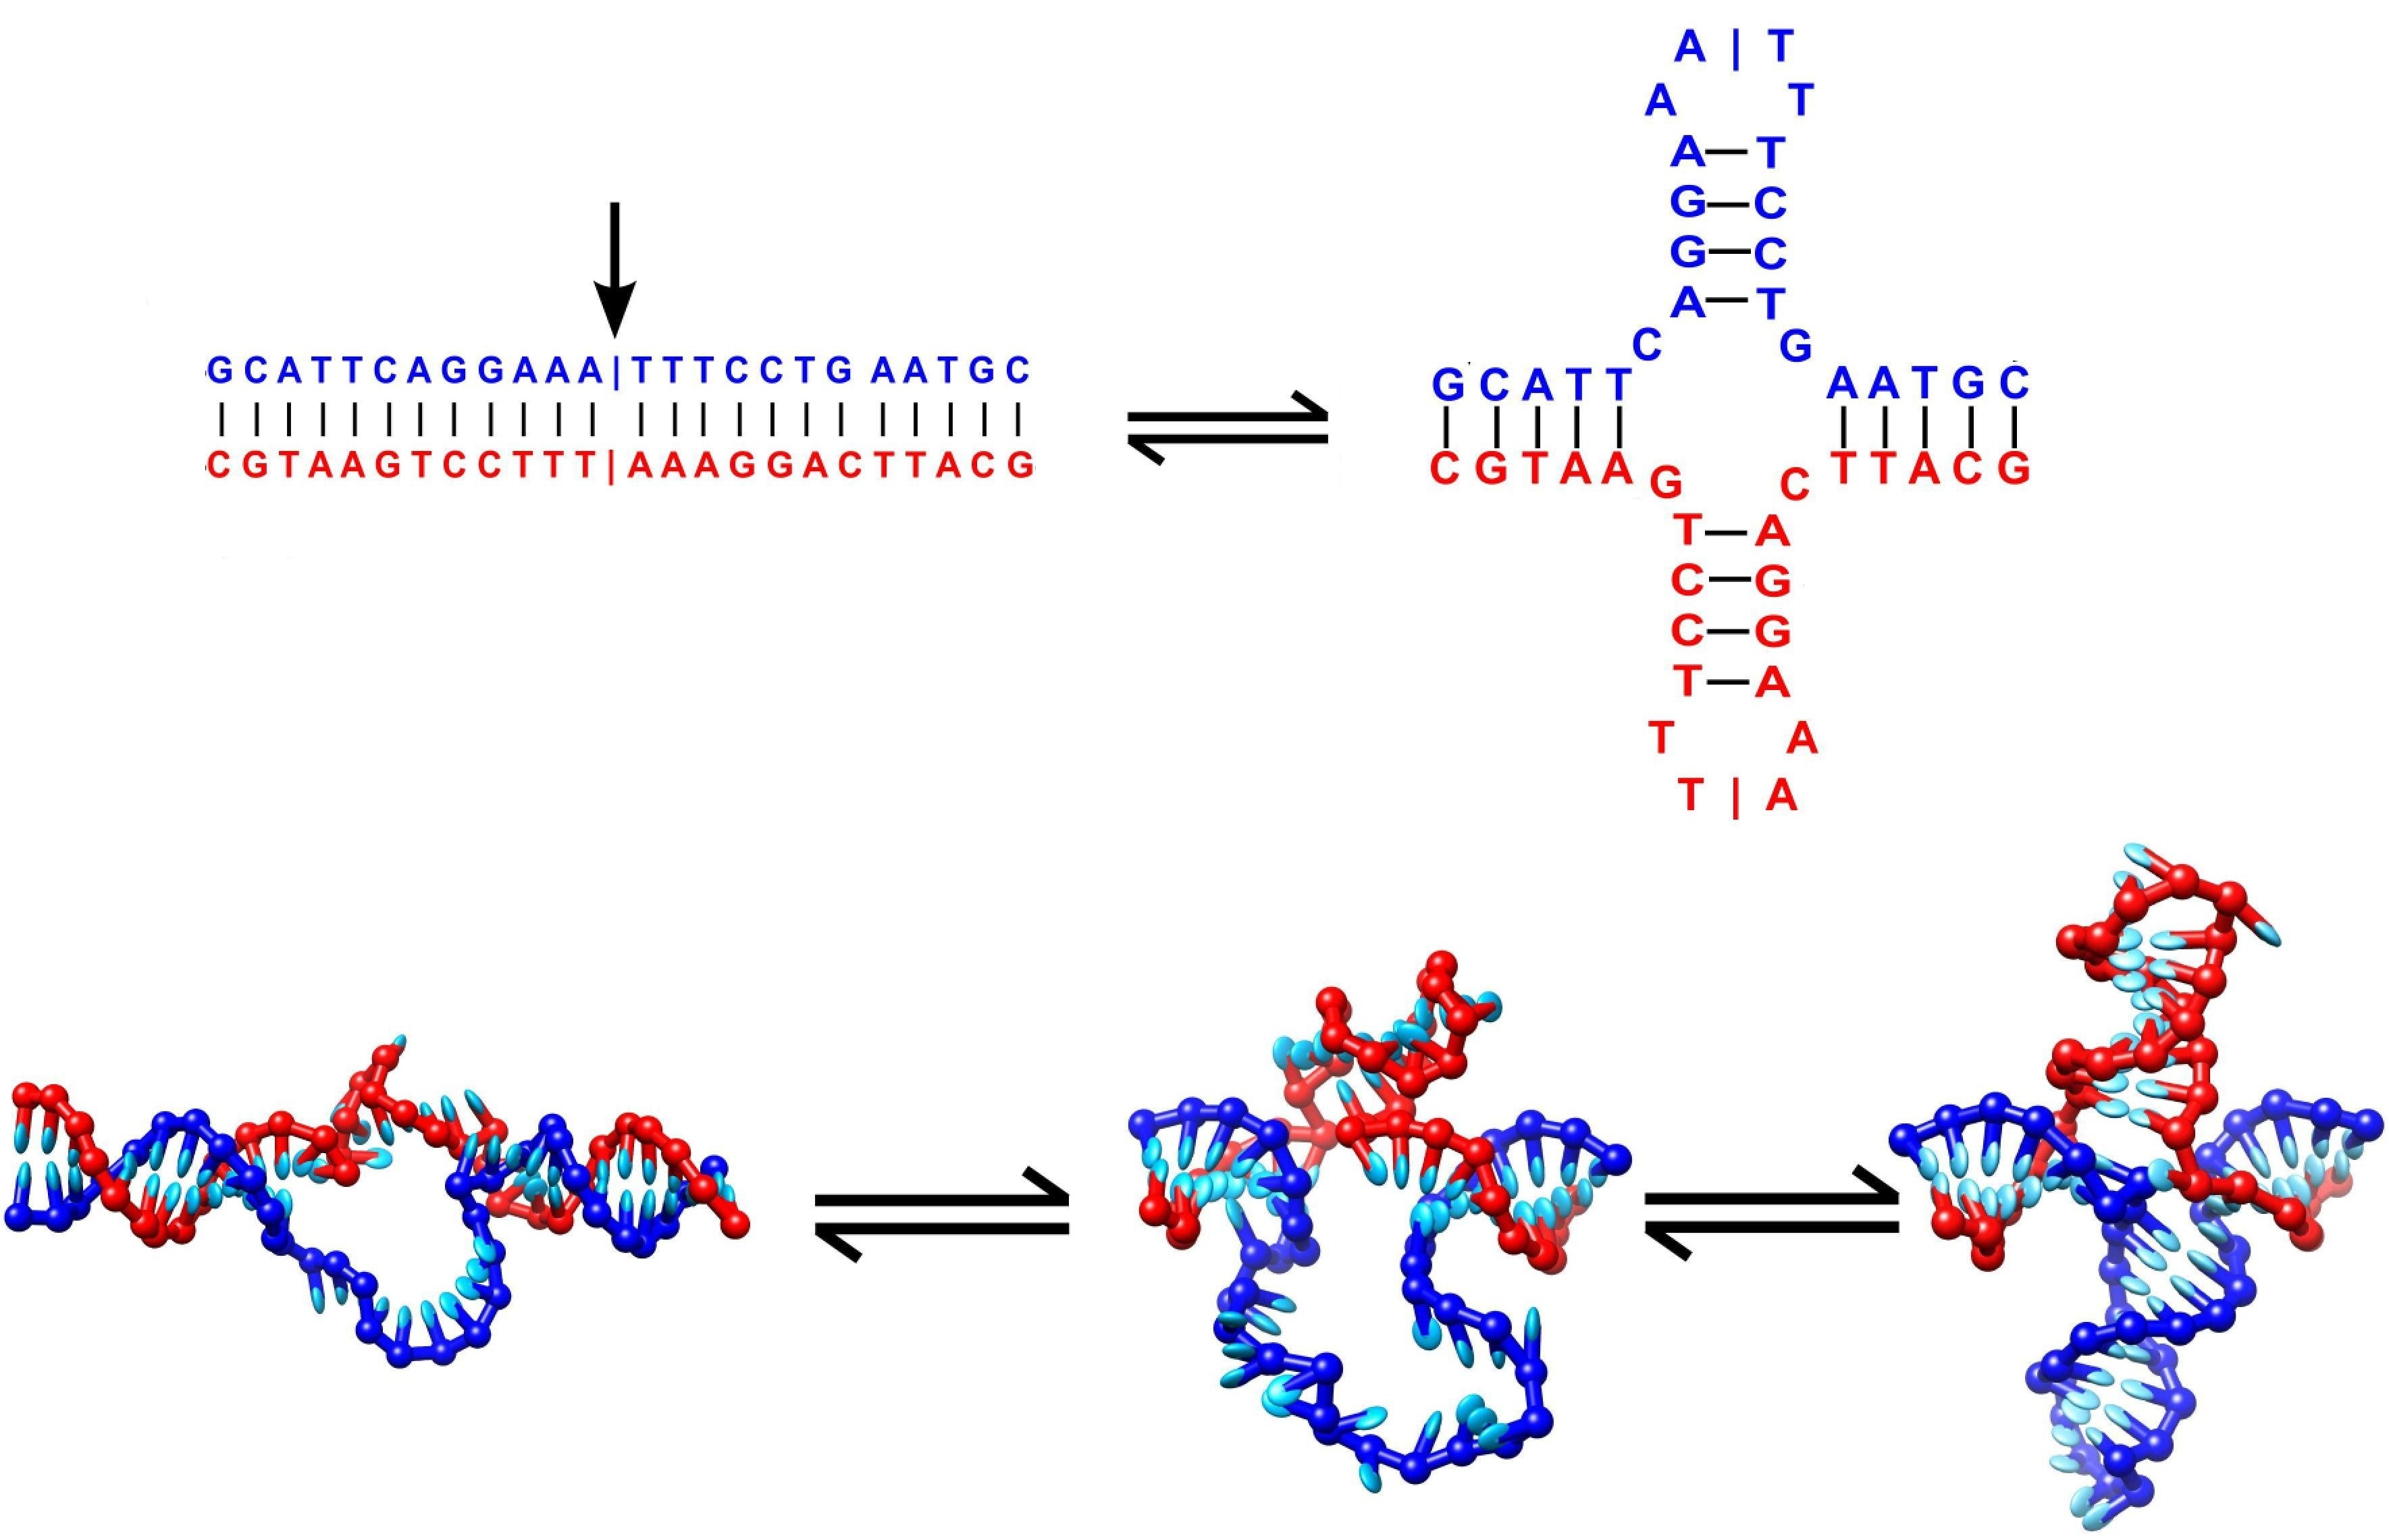
\includegraphics{./poglavlja/uvod/slike/PCA290_A.jpg}
	\caption{Stvaranja ukosnica iz palindroma u DNA nizu
		prikazano pomoću slovčanog i molekularnog
		prikaza DNA niza (izvor \cite{dna_cruciforms}).
		Strelica označava centar palindroma.}
		\label{uvod:fig:ukosnice}
\end{figure}

Budući da su palindromi značajni za funkcioniranje genoma
koristan bi bio nekakav oblik statističkog testa koji bi
odavao ima li palindroma određene duljine značajno više ili manje
od očekivanog broja unutar nekog npr. roda koji se proučava.
Iskaz rezultata koji omogućavaju konstrukciju takvog testa
bit će prezentiran u poglavlju \ref{ch:palindromi} ovog doktorskog rada.


\section*{Doprinosi doktorskog rada}
\addcontentsline{toc}{section}{Doprinosi doktorskog rada}

\begin{itemize}[label=$\bullet$]
	\item{
		Definiran je novi model nizova znakova pomoću
		blokova koji se periodično ponavljaju ili 
		zadržavaju fiksan omjer porastom duljine niza.
		Distribucije znakova unutar blokova su
		jednake, ali ne i nužno iste među blokovima.
		Iskazan je i dokazan teorem o asimptotskoj
		normalnosti broja palindroma fiksne duljine
		u takvim nizovima uz uvjet nezavisnosti.
		Dani su uvjeti na 
		odgovarajuće procjenitelje
		za primjenu na nizovima
		kod kojih treba procjeniti parametre.
	}
\end{itemize}

\section*{Pregled doktorskog rada po poglavljima}
\addcontentsline{toc}{section}{Pregled doktorskog rada po poglavljima}

Prvo poglavlje naslovljeno {\glqq}Pregled poznatih rezultata
i tehničkih metoda'' prezentira neke od najvažnijih
ideja, rezultata i tehničkih metoda koje će biti
potrebne u daljnjim poglavljima kao motivacija
ili tehnički alat. 

U drugom poglavlju  naslovljenom
{\glqq}Distribucija broja palindroma u nizovima znakova''
iskazan je i dokazan teorem o asimptotskoj normalnosti
broja palindroma u nizu znakova modeliranog blokovima.
Dopuštena su dva oblika blokova (periodično ponavljajući
te fiksnog omjera unutar niza) s proizvoljnim
distribucijama znakova unutar blokova.
Nezavisnost svih znakova se pretpostavlja.
Također, dani su uvjeti na procjenitelje za
očekivanje i varijancu pri korištenju asimptotske
normalnosti na nizove kod kojih je potrebno procjeniti
parametre modela. Iznesene su i formule 
za očekivanje i kovarijance palindroma s
proizvoljnim distribucijama. Primjerom primjene
rezultata na stvaran DNA niz prikazana je 
razlika između n.j.d modela te modela s blokovima.
Kvaliteta aproksimacije prezentirana je rezultatima
simulacijske studije.
Na kraju poglavlja dane su određene
primjedbe i zaključak.

\section*{Oznake, kratice i slično}
\addcontentsline{toc}{section}{Oznake, kratice i slično}

Pojmovi koji se prvi put spominju i od značaja su u ostatku
doktorskog rada podebljani su i u kurzivu:
\be{tenzor}, \be{procjenitelj}, \ldots.

\emph{Skalari} će se označavati malim slovima engleske ili 
grčke abecede: $a,b,c,\gamma,\ldots$.

\emph{Vektori} će se označavati malim podebljanim slovima engleske
abecede, a njihovi elementi koristit će indekse.
Na primjer, $v_i$ je $i$-ti element vektora
$\tv{v}=(v_i)_{i=1}^{n}=(v_1,\cdots,v_n)$.
U rijetkim slučajevima, zbog lakše preglednosti,
koristit će se i oznaka $v[i]$ za elemente vektora.

\emph{Matrice} će se označavati velikim slovima engleske
abecede: $\tmatrix{A},\tmatrix{B},\tmatrix{C},\ldots$.
Matrični elementi označavat će se sa
$M_{i,j}=M_{ij}$ ili s $M[i,j]$. Iznimno
će se elementi matrice označavati drukčije
(zadržavajući sintaksu i semantiku) kada
elementima definiramo matricu, npr. $M=[m_{ij}]$.
Za danu matricu $M$
$i$-ti redak će se označavati s $M_{i,:}$ ili $M[i,:]$,
a $j$-ti stupac s $M_{:,j}$ ili $M[:,j]$.


\emph{Tenzori} će se označavati velikim podebljanim slovima
engleske abecede: $\ttenzor{X}, \ttenzor{Y}, \ttenzor{Z},\ldots$.
Elementi tenzora $\ttenzor{X}$ označavat
će se sa $\ttenzor{X}(i_{1},\cdots,i_{n})$. Kada je vektor male dimenzije
ponekad će se koristiti i oznaka $\ttenzor{X}_{i,j,k}=\ttenzor{X}_{ijk}$
za elemente tenzora.

\emph{Slučajne varijable} će se označavati velikim slovima
engleske abecede: $\tsvar{X}, \tsvar{Y}, \tsvar{Z},\ldots$.
Budući da izrazi koji sadrže slučajne varijable uglavnom neće sadržavati
i matrice dvosmislenost ne bi trebala biti problem.

\emph{Slučajni vektori} će se označavati velikim podebljanim slovima
engl. abecede: $\tsvek{X}, \tsvek{Y}, \ldots$.
Budući da izrazi koji sadrže slučajne vektore  neće sadržavati
i tenzore dvosmislenost ne bi trebala biti problem.
Često će se pisati $\tsvek{X} \in K$ da bi se istaknulo
da je kodomena slučajnog vektora $\tsvek{X}$ jednaka $K$.
Da slučajan vektor $\tsvek{X}$ pripada nekoj vjerojatnosnoj
razdiobi $\eta$ označavat će se sa $\tsvek{X}\sim \eta$.
Specifično će ponekad za diskretne distribucije oznaka biti
\[
	\tsvar{X} \sim
	\begin{pmatrix}
	a_1 & a_2 & a_3 & \cdots & a_K \\
	p_{1} & p_{2} & p_{3} & \cdots & p_{K} \\
	\end{pmatrix}
\]
kada se bude htjelo naglasiti koji su mogući ishodi slučajne varijable $X$
($\vP (\tsvar{X} = a_k) = p_{k}$ za sve $k \leq K$). 


\emph{Nizovi znakova} označavat će se velikim slovima 
koristeći efekt malog verzala (engl. \textit{small-caps}). 
Tu su mala slova zamijenjena velikim slovima manje veličine,
dok su velika jednaka običnima, primjerice: \nz{Ivan Gundulić},
\nz{matrica} ili \nz{ACGTTTGCA}. Također, u određenim će se
prilikama koristiti i kurziv pri označavanju:
\nzk{Ivan Gundulić}.


\emph{Nizovi} u matematičkom smislu označavat će se zagradama
poput $(a_k)_k$ gdje će se podrazumijevati da je $k \in \setN$.
Ukoliko bude očito po kojem se indeksu niz pomiče često će se pisati
samo $(a_k)$.



% Chapter: Pregled poznatih tehničkih rezultata i metoda
\chapter{Pregled poznatih tehničkih rezultata i metoda}

U ovom će se poglavlju prezentirati neki od poznatih
rezultata koji će biti od pomoći pri
dokazivanju i korištenju tvrdnji vezanih uz područje
interesa ovog doktorskog rada.

Autorov cilj nije 
u ovom poglavlju proći kroz većinu poznate literature
na potrebnim područjima, već izložiti
sažet i razumljiv uvod u potrebne rezultate
te time omogući čitanje doktorskog rada
bez nužnog posezanja za dodatnom literaturom.

Svako potpoglavlje sadrži reference
na dodatnu literaturu koju
zainteresirani čitatelj može konzultirati
za daljnje proučavanje područja.


\section{Konvergencija slučajnih vektora i varijabli}

Za $d$-dimenzionalan slučajan vektor 
$\tsvek{X} = (\tsvar{X_1},\cdots,\tsvar{X_d})$
\be{funkciju distribucije od $\tsvek{X}$}
\index{funkcija distribucije slučajnog vektora}
definiramo sa
$F_{\tsvek{X}}(x) = 
\vP( \tsvek{X} \leq \tv{x} ) =
\vP( \tsvar{X_1} \leq x_1, \cdots, \tsvar{X_d} \leq x_d)$
za sve $\tv{x}=(x_1,\cdots,x_d) \in \mathbb{R}^d$. 
\be{Euklidsku normu}
\index{euklidska norma}
od $\tv{x}=(x_1,\cdots,x_d) \in \mathbb{R}^d$
označavamo s $|\tv{x}| = (x_{1}^{2}+\cdots+x_{d}^{2})^{\sfrac{1}{2}}$.

\begin{defn}
	Za niz slučajnih vektora $(\tsvek{X}_n)$ kažemo da 
	konvergira slučajnom vektoru $\tsvek{X}$
%
\begin{itemize}
	\item[(i)]{\be{gotovo sigurno (g.s.)}
		\index{konvergencija!gotovo sigurno}
		ako vrijedi
		\begin{equation} \label{equ:konvgs}
			\vP( \lim_{n \rightarrow \infty} \tsvek{X}_n = \tsvek{X}) = 1\ .
		\end{equation}
		Tada pišemo $\konvgs{\tsvek{X}_n}{\tsvek{X}}$.
	}
	\item[(ii)]{\be{u srednjem reda r}
		\index{konvergencija!u srednjem reda r}
		ako za neki realan broj $r>0$ te za $\konv{n}{\infty}$ vrijedi
		\begin{equation}\label{equ:konvusr}
			\vE{| \tsvek{X}_n - \tsvek{X} |^r}  \rightarrow 0\ .
		\end{equation}
		Tada pišemo $\konvusr{\tsvek{X}_n}{\tsvek{X}}{r}$.
	}
	\item[(iii)]{\be{po vjerojatnosti}
		\index{konvergencija!po vjerojatnosti}
		ako za svaki $\varepsilon >0$ te za $\konv{n}{\infty}$ vrijedi
		\begin{equation}\label{equ:konvpv}
			\vP \left( | \tsvek{X}_n - \tsvek{X} | > 
			\varepsilon \right) \rightarrow 0 \ .
		\end{equation}
		Tada pišemo $\konvpv{\tsvek{X}_n}{\tsvek{X}}$.
	}
	\item[(iv)]{\be{po distribuciji}
		\index{konvergencija!po distribuciji}
		ako za sve točke $x$ u kojima je funkcija distrubucije
		$F_{\tsvek{X}}$ slučajnog vektora $\tsvek{X}$ 
		neprekidna (u oznaci $\tv{x} \in C(F_{\tsvek{X}})$) vrijedi
		\begin{equation} \label{equ:konvpd}
			F_{\tsvek{X}_n}(\tv{x}) \rightarrow F_{\tsvek{X}}(\tv{x})
		\end{equation}
		kada $n \rightarrow \infty$. Tada pišemo $\konvpd{\tsvek{X}_n}{\tsvek{X}}$.
	}
\end{itemize}
\end{defn}

Razlog isključivanja svih točaka u kojima $F_{\tsvek{X}}$ nije neprekidna, kod
konvergencije po distribuciji, možda se čini viškom. Međutim,
potreban (koristan) je što prikazuje sljedeći primjer.

\begin{primjer_}
	Kažemo da je slučajan vektor $\tsvek{X} \in \mathbb{R}^d$
	\be{koncentriran}
	\index{koncentriran slučajan vektor}
	u točki $\tv{c} \in \mathbb{R}^d$ ako je $\vP( \tsvek{X} = \tv{c} )=1$.
	Neka je $(\tsvar{X}_n) \in \mathbb{R}$  niz slučajnih varijabli
	koncentriranih u točkama $\sfrac{1}{n}$ za $n=1,2,\ldots$
	te neka je $\tsvar{X} \in \mathbb{R}$ koncentrirana u 0. Budući da
	$\sfrac{1}{n}$ konvergira prema 0 kada $\konv{n}{\infty}$, moglo bi se
	očekivati da će vrijediti $\konvpd{\tsvar{X}_n}{\tsvar{X}}$.

	Funkcija distribucije od $\tsvar{X}_n$ dana je sa 
	$F_{\tsvar{X}_n} = \mathbbm{1}_{[\sfrac{1}{n},\infty]}(x)$,
	a od $\tsvar{X}$ sa $F_{\tsvar{X}} (x) = \mathbbm{1}_{[0,\infty]}(x)$.
	Očito vrijedi
	$\konv{F_{\tsvar{X}_n}(x)}{F_{\tsvar{X}}(x)}$ za $x \neq 0$, dok za $x=0$ vrijedi
	$F_{\tsvar{X}_n}(0) = 0$ i $F_{\tsvar{X}} (x) = 1$. Budući da $x \notin C(F_X)$
	uvjeti konvergencije po distribuciji su zadovoljeni.
\end{primjer_}

Sljedeća lema daje karakterizaciju konvergencije gotovo sigurno
iz koje se lakše vidi razlika između konvergencije
gotovo sigurno i konvergencije po vjerojatnosti.

\begin{lem}
	$\konvgs{\tsvek{X}_n}{\tsvek{X}}$ ako i samo ako za svaki
	$\varepsilon >0$ vrijedi
	\begin{equation} \label{equ:karakterizacijakonvgs}
		\vP( |\tsvek{X}_k - \tsvek{X}| < \varepsilon,\ \forall k \geq n) \rightarrow 1
	\end{equation}
	kada $\konv{n}{\infty}$.
\end{lem}

Riječima razliku možemo opisati na sljedeći način:
za konvergenciju po vjerojatnosti potrebno je da za svaki $\varepsilon >0$
vjerojatnost da će se $\tsvek{X}_n$ nalaziti unutar $\varepsilon$ odmaka od 
$\tsvek{X}$ teži
prema 1 dok je kod konvergencije gotovo sigurno potrebno da za svaki
$\varepsilon >0$ vjerojatnost da $\tsvek{X}_k$ ostane unutar $\varepsilon$ odmaka
od $\tsvek{X}$ za svaki $k \geq n$ teži prema 1 kada $n$ teži prema beskonačnosti.

Odnose među tipovima konvergencija slučajnih varijabli daje sljedeći teorem.

\begin{tm} \label{tm:vezemedjukonvergencijama}
	Za niz slučajnih vektora $(\tsvek{X}_n)$ i slučajan vektor $\tsvek{X}$ vrijedi
	\begin{itemize}
		\item[(i)]{ $\konvgs{\tsvek{X}_n}{\tsvek{X}} 
			\implies \konvpv{\tsvek{X}_n}{\tsvek{X}}$ }
		\item[(ii)]{ $\konvusr{\tsvek{X}_n}{\tsvek{X}}{r}
			\implies \konvpv{\tsvek{X}_n}{\tsvek{X}}$ }
		\item[(iii)]{ $\konvpv{\tsvek{X}_n}{\tsvek{X}} 
			\implies \konvpd{\tsvek{X}_n}{\tsvek{X}}$ }
	\end{itemize}
\end{tm}

Obrati ne vrijede nužno kao što pokazuju sljedeći primjeri.

\begin{primjer_}
	Po definiciji konvergencije po distribuciji slučajne varijable $\tsvar{X}_n$
	ne moraju biti definirane na istom vjerojatnom prostoru
	kao i njihov limes $\tsvar{X}$ pa time ne možemo ni računati
	uvjet konvergencije po vjerojatnosti (\ref{equ:konvpv}).

	Čak i ako su $\tsvar{X}_n$ i $\tsvar{X}$ definirane na istom vjerojatnosnom prostoru
	konvergencija po distribuciji ne mora povlačiti konvergenciju po
	vjerojatnosti. Neka su $\tsvar{X}_n \sim N(0,1)$  nezavisne i jednako distribuirane
	($\tsvar{X}_n$ su normalne slučajne varijable s očekivanjem 0 i varijancom jednakom 1).
	Tada vrijedi $\konvpd{\tsvar{X}_n}{\tsvar{X}_1}$ dok
	$\nkonvpv{\tsvar{X}_n}{\tsvar{X}_1}$.
\end{primjer_}

\begin{primjer_}
	Neka je $\tsvar{Z}$ slučajna varijabla uniformno distribuirana na intervalu $(0,1)$,
	odnosno $\tsvar{Z} \sim U([0,1])$ i neka su 
	$\tsvar{X}_1=1$,
	$\tsvar{X}_2 = \mathbbm{1}_{[0,\sfrac{1}{2}]}(\tsvar{Z})$,
	$\tsvar{X}_3 = \mathbbm{1}_{[\sfrac{1}{2},1]}(\tsvar{Z})$,
	$\tsvar{X}_4 = \mathbbm{1}_{[0,\sfrac{1}{4}]}(\tsvar{Z})$,\ldots.
	Odnosno, ako je $n=2^k + m$, gdje je $0 \leq m \leq 2^k$ i $k \geq 0$, tada
	je $\tsvar{X}_n = \mathbbm{1}_{[m 2^{-k}, (m+1) 2^{-k})}(Z)$.
	Očito $(\tsvar{X}_n)$ ne
	konvergira za bilo koji $Z \in [0,1)$ te time 
	$\nkonvgs{\tsvar{X}_n}{\tsvar{X}}$.
	Međutim, $\konvusr{\tsvar{X}_n}{0}{r}$ za svaki $r>0$ i $\konvpv{\tsvar{X}_n}{0}$.
\end{primjer_}

\begin{primjer_}
	Neka su $\tsvar{Z} \sim U([0,1])$ i $\tsvar{X}_n = 2^n \mathbbm{1}_{[0,\sfrac{1}{n}]}(\tsvar{Z})$.
	Tada $\vE{ |\tsvar{X}_n|^r } = \frac{2^{nr}}{n} \rightarrow \infty$ pa vrijedi
	$\nkonvusr{\tsvar{X}_n}{0}{r}$ za svaki $r>0$. Međutim, $\konvgs{\tsvar{X}_n}{0}$
	($\{ \lim_{n\rightarrow \infty} \tsvar{X}_n = 0\} = \{\tsvar{Z} >0 \}$ i
	$\vP(\tsvar{Z}>0) = 1$) i $\konvpv{\tsvar{X}_n}{0}$
	(ako je $0 < \varepsilon < 1$, $\vP(|\tsvar{X}_n| > \varepsilon) =
	P(\tsvar{X}_n = 2^n) = \sfrac{1}{n} \rightarrow 0)$.
\end{primjer_}

Iako obrati u Teoremu \ref{tm:vezemedjukonvergencijama}
ne vrijede nužno, postoje dovoljni uvjeti kada obrati vrijede.
Isti su dani sljedećim teoremom. 

\begin{tm} Neka je $\tsvek{c}$ koncentriran slučajni vektor u $\mathbb{R}^d$.
	Tada vrijedi
	\begin{itemize}
		\item[(i)]{ $\konvpd{\tsvek{X}_n}{\tsvek{c}} \implies
			\konvpv{\tsvek{X}_n}{\tsvek{c}}$. }
		\item[(ii)]{Ako $\konvgs{\tsvek{X}_n}{\tsvek{X}}$ i 
			$|\tsvek{X}_n|^r \leq \tsvar{Z}$
			za neki $r>0$ i slučajnu varijablu $\tsvar{Z}$ sa
			$\vE{\tsvar{Z}} < \infty$
			tada vrijedi $\konvusr{\tsvek{X}_n}{\tsvek{X}}{r}$.}
		\item[(iii)]{[Scheff\'{e} (1947.)] Ako $\konvgs{\tsvek{X}_n}{\tsvek{X}}$,
			$\tsvek{X}_n \geq 0$ i 
			$\konv{\vE{\tsvek{X}_n}}{\vE{\tsvek{X}}} < \infty$ tada
			$\konvusr{\tsvek{X}_n}{\tsvek{X}}{1}$. }
		\item[(iv)]{$\konvpv{\tsvek{X}_n}{\tsvek{X}}$ 
			ako i samo ako svaki niz prirodnih
			brojeva $(a_k)$ ima podniz $(a_{p(k)})$
			takav da $\konvgs{\tsvek{X}_{a_{p(k)}}}{\tsvek{X}}$
			kada $\konv{k}{\infty}$. }
	\end{itemize}

\end{tm}

Za funkciju $g:\setR^d \rightarrow \mathbb{R}$ kažemo da
\be{iščezava}
\index{iščezavajuća funkcija na kompaktu}
izvan kompakta ako postoji kompaktan skup $K \subset \mathbb{R}^d$
takav da vrijedi $g(\tv{x})=0$ za svaki $\tv{x} \notin K$.

Veza između konvergencije po distribuciji niza slučajnih vektora
i konvergencije po očekivanju funkcija tih vektora dana je
sljedećim teoremom.

\begin{tm}
	Sljedeći su uvjeti ekvivalentni
	\begin{itemize}
		\item[(i)]{$\konvpd{\tsvek{X}_n}{\tsvek{X}}$}
		\item[(ii)]{$\konv{\vE{g(\tsvek{X}_n)}}{\vE{g(\tsvek{X})}}$ za svaku neprekidnu
		funkciju $g$ koja iščezava izvan kompakta.}
		\item[(iii)]{$\konv{\vE{g(\tsvek{X}_n)}}{\vE{g(\tsvek{X})}}$ za svaku
		ograničenu neprekidnu funkciju $g$.}
		\item[(iv)]{$\konv{\vE{g(\tsvek{X}_n)}}{\vE{g(\tsvek{X})}}$ za svaku ograničenu izmjerivu funkciju
			$g$ takvu da vrijedi $\vP(\tsvek{X} \in C(g))=1$.}
	\end{itemize}
\end{tm}

Nekoliko korisnih pravila za rad s konvergencijom po vjerojatnosti
dano je sljedećom propozicijom.

\begin{pro}
	\label{pro:pravilazakonvpv}
	Pretpostavimo da za nizove slučajnih varijabli
	$(\tsvar{X}_n)$ i $(\tsvar{Y}_n)$
	i neke
	konstante $a,b \in \mathbb{R}$ vrijedi
	$\konvpv{\tsvar{X}_n}{a}$, $\konvpv{\tsvar{Y}_n}{b}$ 
	te neka je $c \in \mathbb{R}$ neka konstanta.
	Tada vrijedi
	\begin{flalign*}
		(i) \quad & \konvpv{cX_n}{ca} \ , & \\
		(ii) \quad & \konvpv{X_n + Y_n}{a+b} \ , &\\
		(iii) \quad & \konvpv{X_n Y_n}{a b} \ , &\\
		(iv) \quad & \konvpv{\frac{X_n}{Y_n}}{\frac{a}{b}}
		\quad \text{za } b \neq 0 \ .
		& \\
	\end{flalign*}
\end{pro}

Za nizove slučajnih vektora $(\tsvek{X}_n)$ i $(\tsvek{Y}_n)$ kažemo da su 
$\be{asimptotski ekvivalentni}$
\index{asimptotska ekvivalencija}
ako vrijedi $\konvpv{(\tsvek{X}_n-\tsvek{Y}_n)}{0}$ kada $\konv{n}{\infty}$.

Čest problem u teoriji velikih uzoraka (eng. \emph{large sample theory}) je sljedeći:
za dani niz slučajnih vektora $(\tsvek{X}_n)$ i dani limes po distribuciji $\tsvek{X}$ 
($\konvpd{\tsvek{X}_n}{\tsvek{X}}$) 
treba odrediti limes po distribuciji od $(f(\tsvek{X}_n))$ za neku
funkciju $f$. Sljedeći teoremi prezentiraju neke od rezultata
kojima se rješavaju takvi problemi.

\begin{tm} \label{tm:konvpdfunkcijavektora}
	{\hspace{\stretch{1}}} \nopagebreak
	\begin{itemize}
		\item[(i)]{Ako vrijedi $\tsvek{X}_n \in \mathbb{R}^d$ i 
			$\konvpd{\tsvek{X}_n}{\tsvek{X}}$
			te je funkcija $f:\setR^d \rightarrow \mathbb{R}^k$
			takva da $\vP(\tsvek{X} \in C(f)) = 1$ 
			tada slijedi $\konvpd{f(\tsvek{X}_n)}{f(\tsvek{X})}$}
		\item[(ii)]{Ako $\konvpd{\tsvek{X}_n}{\tsvek{X}}$ i
			$\konvpv{(\tsvek{X}_n-\tsvek{Y}_n)}{0}$ 
			tada
			$\konvpd{\tsvek{Y}_n}{\tsvek{X}}$.}
		\item[(iii)]{Ako vrijedi $\tsvek{X}_n \in \mathbb{R}^d$,
			$\tsvek{Y}_n \in \mathbb{R}^k$,
			$\konvpd{\tsvek{X}_n}{\tsvek{X}}$,
			$\konvpd{\tsvek{Y}_n}{\tv{c}}$ tada
			\begin{equation}
				\konvpd{
					\begin{pmatrix}
						\tsvek{X}_n \\
						\tsvek{Y}_n \\
					\end{pmatrix}
				}{
					\begin{pmatrix}
						\tsvek{X} \\
						\tv{c} \\
					\end{pmatrix}
				}
			\end{equation}
		}
	\end{itemize}
\end{tm}

U prethodnom teoremu s
$
\begin{pmatrix}
	\tsvek{X}_n \\
	\tsvek{Y}_n \\
\end{pmatrix}
$
označili smo vektor iz $\mathbb{R}^{d+k}$ kojem je prvih $d$ elemenata
dano s $\tsvek{X}_n$, a zadnjih $k$ s $\tsvek{Y}_n$, te sa $\tv{c}$
neki koncentrirani slučajni vektor u $\setR^k$.

\begin{primjer_}
	Neka je $\tsvar{X} \sim N(0,1)$ i $\konvpd{\tsvar{X}_n}{\tsvar{X}}$.
	Tada za funkciju
	$f(x)=x^2$ po Teoremu \ref{tm:konvpdfunkcijavektora}
	(dio (i)) slijedi $\konvpd{\tsvar{X}_{n}^{2}}{\tsvar{X}^2}$ budući da je
	$f$ neprekidna. Budući je $\tsvar{X}^2 \sim \chi_{1}^{2}$ kada je
	$\tsvar{X} \sim N(0,1)$ dobivamo $\konvpd{\tsvar{X}_{n}^{2}}{\chi_{1}^{2}}$.
\end{primjer_}

\begin{primjer_}
	Pogledajmo primjer gdje prekidnost funkcije stvara probleme.
	Neka je $\tsvar{X}_n = \sfrac{1}{n}$ i 
	\[
		f(x) = 
		\begin{cases}
			1, & x>0 \\
			0, & x \leq 0
		\end{cases}
	\]
	Tada $\konvpd{\tsvar{X}_n}{0}$, ali $\nkonvpd{f(\tsvar{X}_n)}{f(0)}$.

\end{primjer_}

\begin{primjer_}
	Dio (iii) teorema \ref{tm:konvpdfunkcijavektora} ne može se
	unaprijediti pretpostavljajući da $\konvpd{\tsvek{Y}_n}{\tsvek{Y}}$ 
	te zaključivši
	$
	\konvpd{
		\begin{pmatrix}
			\tsvek{X}_n \\
			\tsvek{Y}_n \\
		\end{pmatrix}
	}{
		\begin{pmatrix}
			\tsvek{X} \\
			\tsvek{Y} \\
		\end{pmatrix}
	}
	$.
	Uzmimo $\tsvar{X} \sim U([0,1])$ i $\tsvar{X}_n=\tsvar{X}$
	za svaki $n \in \mathbb{N}$,
	$\tsvar{Y}_n = \tsvar{X}$ za $n$ neparan te $\tsvar{Y}_n=1-\tsvar{X}$
	za $n$ paran. Tada
	$\konvpd{\tsvar{X}_n}{\tsvar{X}}$ i 
	$\konvpd{\tsvar{Y}_n}{U([0,1])}$, ali
	$
		\begin{pmatrix}
			\tsvar{X}_n \\
			\tsvar{Y}_n \\
		\end{pmatrix}
	$
	ne konvergira po distribuciji.
\end{primjer_}

Izrazito važna posljedica teorema \ref{tm:konvpdfunkcijavektora}
dana je sljedećim korolarom.

\begin{kor}
	\label{kor:konvpdzajednickogvektora}
	Ako vrijedi $\tsvek{X}_n \in \mathbb{R}^d$,
	$\konvpd{\tsvek{X}_n}{\tsvek{X}}$,
	$\tsvek{Y}_n \in \mathbb{R}^k$, 
	$\konvpd{\tsvek{Y}_n}{\tv{c}}$
	te je funkcija $f:\mathbb{R}^{d+k} \rightarrow \mathbb{R}^r$
	takva da 
	$\vP \left(
		\begin{pmatrix}
			\tsvek{X} \\
			\tv{c} \\
		\end{pmatrix}
		\in C(f) \right) = 1$ tada slijedi 
	$\konvpd{f(\tsvek{X}_n,\tsvek{Y}_n)}{f(\tsvek{X},\tv{c})}$.
\end{kor}

\begin{primjer_}
	Ako $\konvpd{\tsvek{X}_n}{\tsvek{X}}$ i 
	$\konvpd{\tsvek{Y}_n}{\tv{c}}$ iz korolara
	\ref{kor:konvpdzajednickogvektora}
	slijedi $\konvpd{\tsvek{Y}_{n}^{T} \tsvek{X}_n}{\tv{c}^{T} \tsvek{X}}$ budući da je
	skalarni produkt neprekidna funkcija.
\end{primjer_}

Kod konvergencije po vjerojatnosti vrijede analogna pravila kao
i kod teorema \ref{tm:konvpdfunkcijavektora} osim
što se dio (iii) može pojačati.

\begin{tm}
\label{tm:slutsky}
%\index{Teorem!Slutsky}
	{\hspace{\stretch{1}}} \nopagebreak
	\begin{itemize}
		\item[(i)]{Ako vrijedi $\tsvek{X}_n \in \mathbb{R}^d$,
 			$\tsvek{X} \in \mathbb{R}^d$,
			$\konvpv{\tsvek{X}_n}{\tsvek{X}}$
			te za funkciju $f:\mathbb{R}^d \rightarrow \mathbb{R}^k$
			vrijedi 
			$\vP(\tsvek{X} \in C(f)) = 1$ 
			tada slijedi $\konvpv{f(\tsvek{X}_n)}{f(\tsvek{X})}$.}
		\item[(ii)]{Ako $\konvpv{\tsvek{X}_n}{\tsvek{X}}$
			i $\konvpv{(\tsvek{X}_n-\tsvek{Y}_n)}{0}$ 
			tada $\konvpv{\tsvek{Y}_n}{\tsvek{X}}$.}
		\item[(iii)]{Ako vrijedi $\tsvek{X}_n \in \mathbb{R}^d$,
			$\tsvek{Y}_n \in \mathbb{R}^k$,
			$\konvpv{\tsvek{X}_n}{\tsvek{X}}$,
			$\konvpv{\tsvek{Y}_n}{\tsvek{Y}}$ tada
			\begin{equation}
				\konvpv{
					\begin{pmatrix}
						\tsvek{X}_n \\
						\tsvek{Y}_n \\
					\end{pmatrix}
				}{
					\begin{pmatrix}
						\tsvek{X} \\
						\tsvek{Y} \\
					\end{pmatrix}
				}
			\end{equation}
		}
	\end{itemize}
\end{tm}

Lako se može pokazati da vrijedi i
analogon teoremu \ref{tm:slutsky} za konvergenciju gotovo
sigurno.

Jedna od osnovnih klasa teorema teorije vjerojatnosti
jesu jaki i slabi zakoni velikih brojeva. Ovdje
izdvajamo dva najpoznatija.

\begin{tm}
\label{tm:zvb}
	Neka su $\tsvek{X}$, $\tsvek{X}_1$, $\tsvek{X}_2$, \ldots nezavisni jednako
	distribuirani slučajni vektori te neka je
	$\overline{\tsvek{X}_n} = \frac{1}{n} \sum_{i=1}^{n} \tsvek{X}_i$.
	Tada vrijedi
	\begin{align}
		\text{\be{jaki zakon velikih brojeva:}}
		\quad &
		\konvgs{\overline{\tsvek{X}_n}}{\vE{\tsvek{X}}}
		\Leftrightarrow
		\vE{|\tsvek{X}|} < \infty
		\\
		\text{\be{slabi zakon velikih brojeva:}}
		\quad & 
		\vE{|\tsvek{X}|} < \infty
		\implies
		\konvpv{\overline{\tsvek{X}_n}}{\vE{\tsvek{X}}}
	\end{align}
\end{tm}

\noindent
Vrijednost 
$\overline{\tsvek{X}_n} = \frac{1}{n} \sum_{i=1}^{n} \tsvek{X}_i$
često nazivamo
\be{uzoračkim očekivanjem}.
\index{uzoračko očekivanje}

Opširniji pregled poznatih rezultata,
kao i dokazi odgovarajućih tvrdnji, mogu
se naći u ~\textcite{ferguson_course_1996},
\textcite{sarapa2002vjerojatnost},
\textcite{shiryaev1995probability}
ili
\textcite{allan2012probability}.


\section{$m$-zavisni nizovi slučajnih varijabli}

\begin{defn}
	Za niz slučajnih varijabli $(\tsvar{Y}_n)$ kažemo da je 
	\be{m-zavisan}
	\index{$m$-zavisni nizovi slučajnih varijabli}
	ako su za svaki $s \in \mathbb{N}$
	skupovi slučajnih varijabli 
	$\{\tsvar{Y}_1,\cdots,\tsvar{Y}_s\}$
	i $\{\tsvar{Y}_{m+s+1},\tsvar{Y}_{m+s+2},\cdots\}$ nezavisni.
\end{defn}

Primjetimo da je $m$-zavisnost ekvivalentna nezavisnosti
niza slučajnih varijabli za $m=0$.

\begin{defn}
	Za niz slučajnih varijabli $Y_n$ kažemo da je 
	\be{stacionaran}
	\index{stacionaran niz slučajnih varijabli}
	ako za sve $s,t \in \mathbb{N}$
	distribucija slučajnog vektora $(Y_t,\cdots,Y_{t+s})$
	ne ovisi o $t$.
\end{defn}

Drugim riječima, niz je stacionaran ako distribucija
bilo kojih $s$ sljedećih opažanja ne ovisi o vremenu
početka promatranja.

Pretpostavimo da je $(\tsvar{Y}_i)$ stacionaran
niz $m$-zavisnih 
slučajnih varijabli te sa $\mu = \vE{\tsvar{Y}_1}$ označimo očekivanje od $\tsvar{Y}_1$,
sa $\sigma_{00}  = \vVar{\tsvar{Y}_1}$ varijancu od $Y_1$ i
sa $\sigma_{0i}  = \vCov{\tsvar{Y}_t, \tsvar{Y}_{t+i}}$ kovarijancu
između $\tsvar{Y}_t$ i $\tsvar{Y}_{t+i}$. Vrijednosti su dobro
definirane i neovisne o $t$ zbog stacionarnosti niza.
Također, iz $m$-zavisnosti za $i>m$ slijedi $\sigma_{0i}=0$.
Očekivanja i varijance slučajnih varijabli
$\tsvar{S}_n = \sum_{i=1}^{n} \tsvar{Y}_i$ dane su formulama
%
\begin{gather*}
	\vE{\tsvar{S}_n} = n \mu \ ,\\
	\vVar{\tsvar{S}_n} = \sum_{i=1}^{n} \sum_{j=1}^{n} \vCov{\tsvar{Y}_i,\tsvar{Y}_j} =
	n \sigma_{00} + 2(n-1)\sigma_{01} + \cdots
	2(n-m)\sigma_{0m} \ .
\end{gather*}
%
Za $\konv{n}{\infty}$ vrijedi $\konv{\vVar{\tsvar{S}_n}/n}{\sigma^2}$ gdje
je $\sigma^2 = \sigma_{00} + 2\sigma_{01} + \cdots + 2\sigma_{0m}$
pa je po sljedećem teoremu distribucija od $\tsvar{S}_n$ aproksimativno normalna
s očekivanjem $\mu$ i varijancom $\sigma^2$.

\begin{tm}
	\label{tm:mzavisanstacionarnicgt}
	Neka je $\tsvar{Y}_n$ stacionaran $m$-zavisan niz slučajnih varijabli
	s konačnim varijancama te $\tsvar{S}_n = \sum_{i=1}^{n} \tsvar{Y}_i$.
	Tada vrijedi
	\begin{equation}
		\konvpd{
			\frac{\tsvar{S}_n - \vE{\tsvar{S}_n}}{\sqrt{\vVar{\tsvar{S}_n}}}
		}{
			N(0,1),
		}
	\end{equation}
	odnosno
	\begin{equation}
		\konvpd{
			\frac{\tsvar{S}_n - \mu n}{\sqrt{n}}
		}{
			N(0,\sigma^2).
		}
	\end{equation}
\end{tm}
%
U slučaju kada niz nije stacionaran asimptotska distribucija
je također normalna uz određene uvjete. Za iskaz te
tvrdnje potrebna nam je sljedeća definicija.

\begin{defn}
	Za slučajnu varijablu $\tsvar{X}$ definiramo 
	slučajnu varijablu $\tsvar{X}^{\alpha}$ kao
	\[
		\tsvar{X}^{\alpha} =
		\begin{cases}
			X, & \text{za } |X| \leq \alpha \\
			0, & \text{inače}
		\end{cases}
	\]
	Za $\tsvar{X}^{\alpha}$ kažemo da je 
	\be{odrezana}
	\index{odrezana slučajna varijabla}
	 u $\alpha$.
\end{defn}


Sljedeći nam teorem govori o konvergenciji po distribuciji
trokutastog niza $m$-zavisnih slučajnih varijabli. Dokaz se može
naći u \textcite{orey_central_1958}(Teorem 1).

\begin{tm}[Orey] 
\label{Thm_Orey_1958}
\index{Teorem!Orey}
Neka je $(p(n))$ neopadajući niz pozitivnih prirodnih brojeva
koji teži prema beskonačnosti, $m$ pozitivan prirodan broj
te $\tau$ pozitivan realan broj. Ako vrijede sljedeći
uvjeti:
\begin{itemize}
	\item[(1)]{ $\{\tsvar{X}_{nv}\}$,
		$v=1,\ldots,p(n)$, $n=1,\ldots$ je trokutasti
		niz $m$-zavisnih slučajnih varijabli, }
	%
	\item[(2)]{ $\sum_{v=1}^{p(n)} \vE{\tsvar{X}_{nv}^{\tau}} \rightarrow \alpha$ kada 
		$\konv{n}{\infty}$ ($\tsvar{X}_{nv}^{\tau}$ su slučajne varijable
		$\tsvar{X}_{nv}$ odrezane u $\tau$),}
	%
	\item[(3)]{ $\sum_{v=1}^{p(n)} \sum_{w=1}^{p(n)} 
		\vCov{\tsvar{X}_{nv}^{\tau}, \tsvar{X}_{nw}^{\tau}} \rightarrow \sigma^2$ kada
		$\konv{n}{\infty}$ ,}
	%
	\item[(4)]{ $\sum_{v=1}^{p(n)} 
		\vP(|\tsvar{X}_{nv}| > \epsilon ) \rightarrow 0$  za svaki $\epsilon > 0$ ,}
	%
	\item[(5)]{ $\sum_{v=1}^{p(n)} \vVar{\tsvar{X}_{nv}^{\tau}} = O(1)$ kada
		$\konv{n}{\infty}$ ,}
\end{itemize}
tada za $n\to\infty$ vrijedi
\[ 
	\konvpd{ \sum_{v=1}^{p(n)} \tsvar{X}_{nv} }{  N(\alpha,\sigma^2) } \ .
\]
\end{tm}

Opširniji pregled poznatih rezultata,
kao i dokazi odgovarajućih tvrdnji, mogu
se naći u ~\textcite{ferguson_course_1996}.


\section{Osnovni pojmovi matematičke statistike}

Neka je $\Omega$ neprazan skup, $\mathcal{F}$ $\sigma$-algebra
nad skupom $\Omega$ te $\mathcal{P}$ familija dopuštenih
vjerojatnosnih razdioba nad $(\Omega, \mathcal{F})$
indeksirana nekim parametrom $\theta$:
\[
	\mathcal{P} = \left\{ P_{\tv{\theta}} : \tv{\theta} \in \Theta \right\}
\]
gdje je $\Theta \subset \mathbb{R}^k,$ $\Theta \neq \emptyset$
skup svih dopuštenih vrijednosti
parametra $\theta$ neke vjerojatnosne razdiobe.
Uređenu trojku
$(\Omega, \mathcal{F}, \mathcal{P})$
zovemo 
\be{statistički eksperiment}
\index{statistički eksperiment}
ili
\be{statistički model}.
\index{statistički model}

\begin{defn}
	Slučajni vektor $\tsvek{X}=(\tsvar{X}_1,\ldots,\tsvar{X}_n)$
	čije su komponente nezavisne
	slučajne varijable sa zajedničkom vjerojatnosnom razdiobom,
	tj. za čiju funkciju distribucije vrijedi
	\[
		\vP_\theta (\tsvar{X}_1 \leq x_1, \ldots, \tsvar{X}_n \leq x_n) =
		\vP_\theta (\tsvar{X}_1 \leq x_1) \cdots \vP_\theta(\tsvar{X}_n \leq x_n) \ ,
		\ \forall \theta \in \Theta , \ \forall (x_1,\ldots,x_n) \in \setR^n
	\]	
	nazivamo \be{slučajnim uzorkom}
	\index{slučajni uzorak}
	veličine $n$.
\end{defn}


\begin{defn}
	\be{Procjenitelj}
	\index{procjenitelj}
	nepoznatog parametra $\theta$ je 
	slučajna varijabla $\hat{\tsvar{T}}$, definirana kao 
	funkcija slučajnog uzorka $\tsvek{X}$. Piše se
	\[
		\hat{\tsvar{T}} = h(\tsvek{X}) = h(\tsvar{X}_1,\ldots,\tsvar{X}_n) \ ,
	\]
	gdje je $h$ realna funkcija $n$ realnih varijabli.
\end{defn}

Slučajnu varijablu kao funkciju slučajnog uzorka uobičajeno je
u matematičkoj statistici zvati 
\be{statistikom}
\index{statistika}
pa se može reći da je procjenitelj statistika.

\begin{defn}
	Procjenitelj koji zadovoljava $\mathrm{E}_{\theta} \left(\hat{\tsvar{T}}\right) = \theta$
	zovemo \be{nepristrani procjenitelj}.
	\index{procjenitelj!nepristran}
\end{defn}

Budući da veličina uzorka u primjenama teorije statističkog
zaključivanja  može varirati korisno je
za procjenitelj uvesti i oznaku
\[
	\hat{\tsvar{T}}_n = h(\tsvar{X}_{1},\ldots,\tsvar{X}_{n}),\ n \in \mathbb{N} \ ,
\]
kako bi se istakla i ovisnost o veličini $n$.  Prijašnjom je relacijom
ustvari definiran beskonačan niz slučajnih varijabli
$(\hat{\tsvar{T}}_{n})_{n \in \mathbb{N}}$.

\begin{defn}
	Neka je $\left\{ P_\theta: \theta \in \Theta \right\}$
	familija distribucija te $\tsvek{X} = \left\{ \tsvar{X}_1,\tsvar{X}_2,\ldots \right\}$
	beskonačan slučajan uzorak.
	Za niz procjenitelja $(\tsvar{T}_{n})$ parametra $g(\theta)$ kažemo da je 
	\be{konzistentan}
	\index{procjenitelj!konzistentan}
	za parametar $g(\theta)$ ako vrijedi
	\[
		\hat{T}_{n} \overset{P_\theta}{\longrightarrow} g(\theta), \ 
		\forall \theta \in \Theta \ .
	\]
\end{defn}

%\textcolor{red}{Treba li objašnjavati:
%Kolmogorov-Smirnov test, Chi-kvadrat test, p-vrijednost ???}

\noindent
Opširniji uvod u matematičku statistiku može se naći u
\textcite{pausestatistika} ili \textcite{schervish_theory_1995}.

 


% Chapter: Distribucija broja palindroma u nizovima znakova
\chapter{Distribucija broja palindroma u nizovima znakova}
\label{ch:palindromi}

\section{Uvod}

Riječ palindrom uvriježena je među različitim
nacijama kao izraz za niz znakova koji se
čitaju isto slijeva nadesno i zdesna nalijevo.
Prema hrvatskom jezičnom portalu (\cite{hjp}) definicija bi bila
{\glqq}igra riječi u kojoj se čitanjem jedne riječi ili čitave rečenice 
obrnutim redom dobiva isto značenje kao i pravilnim čitanjem''.
Etimologija same riječi dolazi
iz grčkog \emph{palindromos}: koji trči natrag
(\emph{palin-} + \emph{-drom}).
Vjerojatno je većini poznat iz mozgalica kojima
se djeca zabavljaju u osnovnoj školi poput
{\glqq}Ana voli Milovana''.

Osnovno proširenje pojma palindroma
dolazi iz područja bioinformatike gdje se palindromi
definiraju kao nizovi znakova koji se čitaju slijeva
isto kao i tome komplementarni niz zdesna. 
Komplementarni niz
se dobiva zamjenom slova klasičnim povezivanjem
adenina, citozina, guamina i timina. Odnosno,
\nzdna{A} se mijenja sa \nzdna{T} (i obratno) te
\nzdna{C} sa \nzdna{G} (i obratno). Primjer palindroma u DNA
nizu jest \nzdna{ACTAGT} jer je njegov komplementarni niz
\nzdna{TGATCA}. Lako je uočiti 
da su jedini mogući palindromi
u DNA nizovima oni parne duljine.

Korisnost proučavanja palindroma u DNA nizovima slijedi iz dosadašnjih
istraživanja koja ukazuju na zaključak da su palindromi
u molekuli DNA nužni za funkcioniranje genoma jer se često nalaze u 
bis-djelujućim regijama, ali istovremeno predstavljaju ozbiljnu opasnost
za genetičku stabilnost
(\textcite{lobachev_hairpin-_2007}),
pri čemu genetička nestabilnost palindroma raste 
s njihovom duljinom
(\textcite{nag_140-bp-long_1997}).
Palindromi se nalaze i kao dijelovi regulacijskih sekvenci,
poput operatora
(\textcite{sinden_perfect_1983}),
promotora
(\textcite{thukral_two_1991}),
terminatora 
(\textcite{gomes_evolution_2007})
i ishodišta replikacije
(\textcite{chew_scoring_2005})
te stoga čine nužan dio genetičkog materijala.
Također, zbog definirane simetrije palindromi u DNA nizovima
tvore sekundarne strukture poput strukture ukosnice
čije formiranje tijekom 
replikacije može uzrokovati {\glqq}proklizavanje''
DNA-polimeraze te može zaustaviti replikaciju
(\textcite{waldman_long_1999}).

Višeznačnost palindroma u DNA nizovima potaknula je razna
bioinformatička istraživanja sekvencioniranih genoma s ciljem 
ustanovljivanja broja, duljine i rasporeda svih palindroma. 

Velik dio istraživanja sastoji se od prepoznavanja
sadrži li niz značajno 
više palindroma od očekivanog broja
(\textcite{robin_dna_2005})
pa bi poznavanje distribucije
broja palindroma u unaprijed definiranom vjerojatnosnom
modelu DNA niza bilo od velike koristi.

Osim u bioinformatici palindromi su standardni dio
istraživanja i u diskretnoj matematici
(područje koje se zove kombinatorika nad riječima)
gdje, na primjer, igraju važnu ulogu pri generiranju
Christoffelovih riječi
s primjenama u teoriji brojeva 
(diofantskim aproksimacijama)
(\textcite{lothaire_applied_2005,
fischler_palindromic_2006}).

\section{Povezana istraživanja}
\label{pal:sec:referencework}

Vjerojatnosna svojstva različitih oblika nizova znakova
(riječi) učestali su predmet istraživanja posljednja
dva desetljeća. Povećanjem računalne moći te naročito
probojem osobnih računala analiza nizova znakova,
u prvom redu DNA nizova, postaje moguća te time
i zanimljiva.

Značaj palindroma za različite biološke nizove,
kao što je prikazano u Uvodu, dovodi do potrebe
za kvalitetnim alatima pri analiziranju svojstava
palindroma kao i odnosa između palindroma i 
nizova znakova u kojima se nalaze. Budući
da su palindromi ustvari vrste riječi s posebnom
strukturom, rezultate o vjerojatnosnim svojstvima
riječi većinom je moguće izravno primijeniti
i na palindrome.

U poglavlju {\glqq}Statistike nad riječima s primjenama
na biološkim nizovima'' knjige 
\cite{lothaire_statistics_2005}[poglavlje 6]
izvode se određena svojstva riječi pa time i palindroma.
Za niz znakova pretpostavlja se da je generiran 
homogenim Markovljevim lancem proizvoljnog reda
(n.j.d. slučaj je reda 0)
unoseći time zavisnost među
elementima. Međutim, ista se zavisnost podrazumijeva
za cijeli niz pa se time gubi ideja regija, odnosno
nije moguće modelirati dijelove niza znakova kao
različite regije s različitim distribucijama.
Među prezentiranim rezultatima bitno je spomenuti
da su izneseni rezultati o asimptotskoj distribuciji
broja palindroma kao i odgovarajućim procjeniteljima
za očekivanje i varijancu. Također, dane su ocjene 
kvalitete aproksimacija normalnom i Poissonovom
distribucijom koristeće Steinovu i Chen-Steinovu
metodu. Svi su rezultati dani za homogene modele,
a autori navode da do trenutka pisanja knjige
nisu upoznati sa statističkim rezultatima
nad heterogenim modelima.

Knjiga \textcite{robin_dna_2005} prezentacija je dijela
rezultata (tehnički manje zahtjevnih) spomenutih i u 
knjizi \cite{lothaire_statistics_2005}
uz dodatak ilustracije važnosti aproksimacija broja
palindroma kroz uvod u bioinformatiku.

\textcite{chew_scoring_2005} promatraju problem
određivanja klastera unutar DNA nizova s velikim
(neočekivanim) brojem palindroma.
Kao pomoć pri klasteriranju definiraju tri
različite težine palindroma dajući tim
određenim palindromima prednost nad drugima.
U radu se pretpostavlja homogeni model DNA niza.


\textcite{leung_nonrandom_2005} također promatraju problem određivanja
iznimnih klastera palindroma. U radu se daje dokaz nekih
osnovnih svojstava palindroma u DNA nizovima te
se izvodi aproksimacija pojavljivanja palindroma
Poissonovim procesom za n.j.d. model DNA niza
uz uvjet $p_A=p_T$ i $p_C = p_G$.

Distribucija broja palindroma po različitim regijama
ljudskog genoma empirijski je određena
u \textcite{lu_human_2007}.

U \textcite{chan_importance_2010} prikazana je primjena
računalnih simulacija, definirani su specifični algoritmi,
na određivanje distribucije broja riječi (ne nužno palindroma).

\textcite{robin_numerical_2001} daju numeričku usporedbu
nekoliko aproksimacija distribucije broja riječi
(međusobno i naspram egzaktne distribucije)
u slučajnim nizovima znakova.
Korištene su aproksimacije normalnom i 
složenom Poissonovom razdiobom.
Pretpostavlja se homogeni Markovljev model kao
model niza znakova.

\textcite{zhai_normal_2012} izvode aproksimaciju 
normalnom i složenom Poissonovom razdiobom 
za distribuciju broja riječi kod
NGS (Next generation sequencing) tehnika modeliranja
nizova znakova.

U diplomskom radu \textcite{gacesa_zastupljenost_2011} razvijen je računalni program
za određivanje očekivanog broja palindroma u kodirajućoj DNA. Program se zasniva
na uspoređivanju broja palindroma u zadanom nizu i u računalno generiranim 
nizovima koji se od zadanog niza razlikuju samo po položaju sinonimnih kodona.

Autor ovog doktorskog rada, u koautorstvu s D. Špoljarićem, 
objavio je sažetu verziju
rezultata prezentiranih u ovom poglavlju kao dio rada
\textcite{spoljaric_statistical_2013}.


\section{Matematički model}

U ovom će se potpoglavlju iznijeti matematički
rezultati o palindromima na proizvoljnom konačnom
skupu znakova.

\subsection{Definicija modela}
\label{pal:sec:defmodela}

Neka su slučajne varijable $\tsvar{X}_n$
nezavisne i distribuirane na sljedeći način:
\[
	\tsvar{X}_n \sim
	\begin{pmatrix}
	a_1 & a_2 & a_3 & \cdots & a_K \\
	p_{1}^{(n)} & p_{2}^{(n)} & p_{3}^{(n)} & \cdots & p_{K}^{(n)} \\
	\end{pmatrix}
	\ ,
\]
odnosno $\vP (\tsvar{X}_n = a_k) = p_{k}^{(n)}$ za sve $n \in \setN$,
$k \leq K$. Vrijednosti
$a_i$ predstavljaju znakove neke abecede, a $p_{i}^{(n)}$ vjerojatnosti
pojavljivanja tih znakova na mjestu $n$ u nizu. Skup svih znakova $a_i$
označavat ćemo sa $\mathcal{A} = \{a_1, a_2, \ldots, a_K \}$.

Neka je $\ol{\cdot} : \mathcal{A} \rightarrow \mathcal{A}$ 
bijektivna funkcija
takva da vrijedi $\dol{x} = x $ za svaki $x \in \mathcal{A}$.
Takvu ćemo funkciju nazivati
\be{funkcijom komplementarnosti}.
\index{funkcija!komplementarnosti}
Ukoliko budemo koristili indekse kao u izrazu $\ol{\tsvar{X}_{i+j}}$
često ćemo pisati samo $\ol{\tsvar{X}}_{i+j}$.
Najjednostavniji primjer funkcije komplementarnosti jest identiteta.

\begin{defn}
	\label{df:palindrom}
	Za niz znakova $b_1$, $b_2$,\ldots, $b_M$ iz $\mathcal{A}$
	kažemo da tvori
	\begin{itemize}
		\item[(i)]{
			\be{(paran) palindrom}
			\index{palindrom}
			\index{palindrom!paran}
			veličine $M$ ako je $M$ paran broj te vrijedi
			$$
			b_1 = \ol{b}_M,\ b_2 = \ol{b}_{M-1}, \ldots,
			b_{\frac{M}{2}} = \ol{b}_{\frac{M}{2} +1}
			\ ,$$}
		\item[(ii)]{
			\be{neparan palindrom}
			\index{palindrom!neparan}
			veličine $M$ ako je $M$ neparan broj te vrijedi
			$$
			b_1 = \ol{b}_M,\ b_2 = \ol{b}_{M-1}, \ldots,
			b_{\frac{M-1}{2}} = \ol{b}_{\frac{M+3}{2}},
			b_{\frac{M+1}{2}} = \ol{b}_{\frac{M+1}{2}}
			\ ,$$}
	\end{itemize}
\end{defn}

U ostatku teksta proučavat ćemo parne palindrome te u
rijetkim dijelovima i neparne palindrome.

\begin{napomena_}
	\label{nap:neparnipalindromidentiteta}
	Iz definicije neparnog palindroma vidimo da za centralni
	element mora vrijediti $b_{\frac{M+1}{2}} = \ol{b}_{\frac{M+1}{2}}$.
	Stoga, broj mogućih kombinacija za neparne palindrome
	ovisi o bliskosti funkcije komplementarnosti 
	identiteti $\ol{a}_i = a_i$ za svaki $a_i \in \mathcal{A}$.
	Odnosno, ovisi o broju elemenata od $a_i \in \mathcal{A}$ takvih
	da vrijedi $\ol{a}_i = a_i$.
\end{napomena_}

\begin{primjer_}[{DNA}]
	Poznato je da se DNA nizovi sastoje od četiri slova (A-adenin,
	C-citozin, G-guanin, T-timin) te da se prirodno uparuju
	adenin s timinom te citozin s guaninom.
	U uvodu smo opisali da će palindromi od značaja u DNA nizovima
	biti dani funkcijom komplementarnosti
	$\ol{A}=T$, $\ol{C}=G$, $\ol{G}=C$, $\ol{T}=A$,
	odnosno prirodnim uparivanjem baza.
	Iz napomene \ref{nap:neparnipalindromidentiteta} slijedi
	da se u DNA nizovima ne mogu dobiti neparni palindromi.
	Primjeri parnih palindroma u DNA nizu dani su
	u tablici \ref{tab:primjeripalindromaudna}.
	\begin{table}[!h] 
		\caption{Primjeri palindroma u DNA nizovima}
		\label{tab:primjeripalindromaudna}
		\centering
		\begin{tabular}{rl} \hline
			\nzdna{ACGT} & parni palindrom duljine 4  \\
			\nzdna{ACCGTACGGT} & parni palindrom duljine 10  \\
			\hline
		\end{tabular}
	\end{table}
\end{primjer_}

Definirajmo
\be{blok}
\index{blok!znakova}
znakova kao neprekinuti niz znakova duljine barem jedan.
Točnije, blokom $B$ duljine $L_B$ smatrat ćemo bilo koji niz
slučajnih varijabli oblika $(X_k,\cdots,X_{k+L_B-1})$
te ćemo zbog jednostavnosti koristiti oznaku $X_k\cdots X_{k+L_B-1}$.
Promatrat će se blokovi koji su disjunktni i povezani
(ne postoje elementi između blokova)
te će slučajne varijable unutar svakog bloka biti
jednako distribuirane.

Dva oblika povezivanja blokova su dopuštena
s obzirom na povećanje niza $X_1,\ldots,X_n$ (po $n$):
\begin{itemize}
\item[(T1)]{
	blokovi se mijenjaju zajedno s duljinom
	niza $n$ zadržavajući omjere veličina blokova
	unutar cijelog niza jednakima 
	\begin{table}[!htpb]
	\centering
	\begin{tabular}{|ccc|ccccccc|c|ccccc|}
	  &  $B_1$ &  &  & &  &  $B_2$ &  &  &  &  $B_3$ &  &  &  $B_4$ &  &  \\
	\hline
	\end{tabular}
\end{table}
}
\item[(T2)]{
	blokovi se izmjenjuju periodično, npr. $B_{1}B_{2}B_{3}B_{1}B_{2}B_{3}\ldots$
}
\end{itemize}
Ideja blokova proizlazi iz potrebe da se opišu različiti dijelovi
DNA nizova (npr. \glslink{dnacodingregion}{kodirajuće regije}
i \glslink{dnanoncodingregion}{nekodirajuće regije}) koji
mogu utjecati na broj palindroma budući da distribucije baza
mogu biti različite u različitim blokovima.
Na primjer, regija s visokom frekvencijom baza $A$ i $T$
ima veću vjerojatnost sadržavati velik broj palindroma
od regije s uniformnom razdiobom baza.

U ostatku doktorskog rada podrazumijevat ćemo da su veličine blokova
veće od duljine palindroma od interesa. U primjenama
se takva pretpostavka podrazumijeva budući da su palindromi
od interesa uvijek manji od regija koje opisuju blokovi
(\textcite{lisnic_palindrome_2005}).

Označimo sa $m$ fiksnu duljinu palindroma. Neka slučajna varijabla
$\tsvar{Y}_i^{(m)}$ bude indikator da palindrom duljine $m$ završava na poziciji
(indeksu) $i$ u nizu $\tsvar{X}_1\cdots\tsvar{X}_n$. Odnosno, za $\tsvar{Y}_i$ vrijedi
\begin{equation}
	\label{df:palindromslvar}
	\tsvar{Y}_i^{(m)}=
	\mathbbm{1}_{\{ \ol{\tsvar{X}}_{i} = \tsvar{X}_{i-m+1}\}} \cdot
	\mathbbm{1}_{\{ \ol{\tsvar{X}}_{i-1} = \tsvar{X}_{i-m+2}\}} \cdots
	\mathbbm{1}_{\{ \ol{\tsvar{X}}_{i-\frac{m}{2}+1} = \tsvar{X}_{i-\frac{m}{2}}\}} 
	\ .
\end{equation}

Budući da je duljina palindroma jednaka $m$, slučajne varijable
$\tsvar{Y}_i^{(m)}$ dobro su definirane za $i \geq m$.
Definirajmo sada \be{broj palindroma} duljine $m$ kao slučajnu varijablu
\begin{equation}
	\label{df:brojpalindroma}
	\tsvar{N}_n = \sum_{i=m}^{n} \tsvar{Y}_i^{(m)} \ .
\end{equation}

Ukoliko ubuduće iz konteksta bude jasno o kojoj se duljini palindroma
radi, indeks $m$ će se izostavljati iz $\tsvar{Y}_i^{(m)}$ te će se pisati
samo $\tsvar{Y}_i$.

\subsection{Osnovna svojstva palindroma}

U cijelom ovom potpoglavlju duljina palindroma je
fiksna i označava se sa $m$.
Iz definicije slučajnih varijabli $\tsvar{Y}_i$ očito je da
je $\tsvar{Y}_m,\ldots,\tsvar{Y}_n$ niz $(m-1)$-zavisnih slučajnih varijabli.

\begin{lem}
\label{pal:lem:meanvarpalindroma}
	Za slučajne varijable $\tsvar{Y}_i$  vrijedi
	\[
		\vP( \tsvar{Y}_i = 1) =
		\prod_{j=1}^{\frac{m}{2}} \left(
		\sum_{x \in \mathcal{A}}
		p_x^{(i-j+1)} p_{\ol{x}}^{(i-m+j)}
		\right)
	\]
\end{lem}

\begin{proof}
	\begin{align*}
		\vP( \tsvar{Y}_i = 1) & = 
		\text{(nezavisnost sl. varijabli $\tsvar{X}_i$)} \\
		& =  \vP( \ol{\tsvar{X}}_i = \tsvar{X}_{i-m+1}) \cdot
		\vP( \ol{\tsvar{X}}_{i-1} = \tsvar{X}_{i-m+2}) \cdots
		\vP( \ol{\tsvar{X}}_{i-\frac{m}{2}+1} = \tsvar{X}_{i-\frac{m}{2}}) \\
		& =
		\left(
		\sum_{x \in \mathcal{A}}
		p_x^{(i)} p_{\ol{x}}^{(i-m+1)}
		\right) \cdot
		\left(
		\sum_{x \in \mathcal{A}}
		p_x^{(i-1)} p_{\ol{x}}^{(i-m+2)}
		\right) \cdots
		\left(
		\sum_{x \in \mathcal{A}}
		p_x^{(i-\frac{m}{2}+1)} p_{\ol{x}}^{(i-\frac{m}{2})}
		\right) \\
		& =
		\prod_{j=1}^{\frac{m}{2}} \left(
		\sum_{x \in \mathcal{A}}
		p_x^{(i-j+1)} p_{\ol{x}}^{(i-m+j)}
		\right) 
	\end{align*}
\end{proof}

\noindent
Budući da su $\tsvar{Y}_i$ Bernoullijeve slučajne varijable
iz prethodne leme slijede jednakosti
\begin{align}
	\vE{|\tsvar{Y}_i|^{r}} &=
	\vE{ \tsvar{Y}_i^{r} } = \vP(\tsvar{Y}_i=1),\ r>0
	\\
	\vVar{\tsvar{Y}_i} &= 
		\prod_{j=1}^{\frac{m}{2}} \left[
		\sum_{x \in \mathcal{A}}
		p_x^{(i-j+1)} p_{\ol{x}}^{(i-m+j)}
		\right]
		\left(
		1 -
		\prod_{j=1}^{\frac{m}{2}} \left[
		\sum_{x \in \mathcal{A}}
		p_x^{(i-j+1)} p_{\ol{x}}^{(i-m+j)}
		\right] 
		\right) 
\end{align}

čime za slučajne varijable $Y_i$  definirane
nad nezavisnim jednako distribuiranim slučajnim 
varijablama $X_i$ vrijedi
\begin{align}
	&
	\label{pal:eqn:meanpalindromanjd}
	\vP(\tsvar{Y}_i = 1) =
		\left(
		\sum_{x \in \mathcal{A}}
		p_x p_{\ol{x}}
		\right)^{\frac{m}{2}} \ , \\
	&
	\label{pal:eqn:varpalindromanjd}
	\vVar{Y_i} = 
		\left(
		\sum_{x \in \mathcal{A}}
		p_x p_{\ol{x}}
		\right)^{\frac{m}{2}}
		\left(
		1-
		\left[
		\sum_{x \in \mathcal{A}}
		p_x p_{\ol{x}}
		\right]^{\frac{m}{2}}
		\right) \ .
\end{align}

Prethodne se jednakosti mogu primijeniti na slučajne varijable $\tsvar{X}_i$ iz
istog bloka budući da su unutar bloka $\tsvar{X}_i$ nezavisne i jednako distribuirane.

Za izvod zatvorene formule za kovarijancu između slučajnih varijabli
$\tsvar{Y}_i$ i $\tsvar{Y}_j$
potrebne su sljedeće leme.

\begin{lem} \label{pal:lem:mixvarijabli}
	Za $u,v \in \mathbb{N}_{0}$, $u+v>1$ vrijedi
	\begin{align}
		& \vP( \tsvar{X}_{i_1} = \cdots = \tsvar{X}_{i_u} 
		= \ol{\tsvar{X}}_{i_{u+1}} = \cdots
		= \ol{\tsvar{X}}_{i_{u+v}}) \nonumber \\
		& \hspace{1em}
		= \sum_{x \in \mathcal{A}}
		p_{x}^{(i_1)}
		p_x^{(i_2)}
		\cdots
		p_x^{(i_u)}
		p_{\ol{x}}^{(i_{u+1})}
		\cdots
		p_{\ol{x}}^{(i_{u+v})}
	\end{align}
\end{lem}
%
\begin{proof}
	Tvrdnja jednostavno slijedi primjenom rastava
	na uvjetne vjerojatnosti.
\end{proof}

\begin{napomena_} \label{pal:nap:njdmixvarijabli}
	Za n.j.d. slučajne varijable $X_i$ jednakost iz prethodne leme
	prelazi u
	\begin{equation}
		\vP (\tsvar{X}_{i_1} = \cdots = \tsvar{X}_{i_p} 
		= \ol{\tsvar{X}}_{i_{u+1}} = \cdots
		= \ol{\tsvar{X}}_{i_{u+v}}) 
		= \sum_{x \in \mathcal{A}}
		\left( p_{x}^{(i_1)} \right)^{u}
		\left( p_{\ol{x}}^{(i_1)} \right)^{v}
	\end{equation}
\end{napomena_}

\noindent
Za palindrom
$z_i = x_{i-m+1} \cdots x_{i}$ \be{desni centar}
definiramo kao element $x_{i-\frac{m}{2}+1}$
te ga označavamo s $C_{z_i}^{D}$.
\be{Lijevi centar} definiramo kao element $x_{i-\frac{m}{2}}$
te ga označavamo s 
$C_{z_i}^{L}$.

Standardne intervalne oznake koristit ćemo na sljedeći
način: 
sa $\left<x_i,x_j\right>$ definiramo niz elemenata od $x_{i+1}$ do
$x_{j-1}$; 
sa $\left<x_i,x_j\right]$ definiramo niz elemenata od $x_{i+1}$ do
$x_{j}$; 
sa $\left[x_i,x_j\right>$ definiramo niz elemenata od $x_{i}$ do
$x_{j-1}$; 
sa $\left[x_i,x_j\right]$ definiramo niz elemenata od $x_{i}$ do
$x_{j}$. Oznake intervala koristit ćemo ponekad
i kao oznake za skupove ne mareći za redoslijed 
znakova koje sadrže.

Nad intervalima ćemo pisati \~{} kao oznaku
za niz komplementiranih znakova originalnog
niza napisan u obrnutom smjeru. Odnosno,
$$
\ol{[x_i,x_j]} := \ol{x}_j \ol{x}_{j-1} \cdots \ol{x}_i \ .
$$

\begin{lem}
	\label{lem:opresjekupalindroma}
	Dva palindroma $z_i$, $z_j$, $j>i$ koja se sijeku
	($j-i < m$)
	u potpunosti su određena elementima iz $\left[C_{z_i}^{D},C_{z_j}^{D}\right>$.
\end{lem}

\begin{proof}
	
	Ilustrirajmo dokaz opisom pravila kojim su elementi
	određeni kroz slike.
	Neka su zadani samo elementi skupa
	$\left[C_{z_i}^{D},C_{z_j}^{D}\right>$ (elementi ispunjeni crnom bojom).

	\begin{figure}[htb!]
	\centering%
	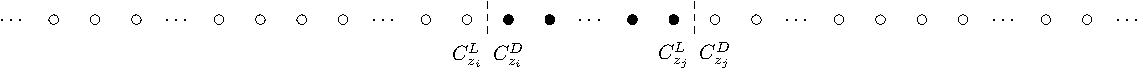
\includegraphics[scale = 0.8]{poglavlja/palindromi/slike/odredjenost-korak0-crop.pdf}
	\end{figure}

	Koristeći pravilo komplementarnosti elemenata palindroma
	s obzirom na centar palindroma $z_j$ (puna linija) 
	poznati elementi jedinstveno određuju nove elemente.

	\begin{figure}[htb!]
	\centering%
	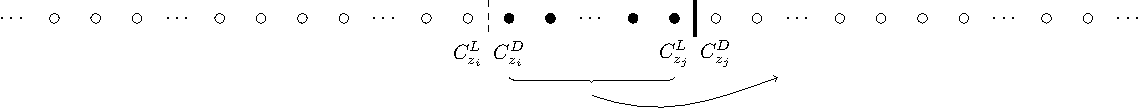
\includegraphics[scale = 0.8]{poglavlja/palindromi/slike/odredjenost-korak1-crop.pdf}
	\end{figure}

	Koristeći komplementarnost elemenata palindroma $z_i$ s
	obzirom na centar palindroma $z_i$ (puna linija)
	poznati elementi jedinstveno određuju nove elemente.

	\begin{figure}[htb!]
	\centering%
	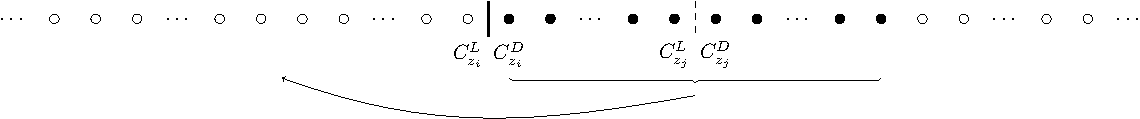
\includegraphics[scale = 0.8]{poglavlja/palindromi/slike/odredjenost-korak2-crop.pdf}
	\end{figure}

	Isti se pristup (naizmjenično korištenje komplementarnosti elemenata palindroma)
	sada primjenjuje sve dok se cijeli palindromi ne ispune.

\end{proof}

\begin{napomena_}
	\label{pal:nap:oblikpresjecenihpalindroma}
	Iz dokaza leme \ref{lem:opresjekupalindroma} slijedi da za dva palindroma
	$z_i$ i $z_j$ koja se sijeku varijable $(X_{i-m+1},\cdots,X_{j})$
	imaju sljedeću strukturu:

\begin{center}
\begin{tabular}{ttttttttttt}
	&
	$\underbrace{\qquad X_{i-m+1} \cdots X_{i-m+r}}_{\lambda \text{ ili } \ol{\lambda}}$
	&
	$\cdots\lambda$
	&
	$\ol{\lambda}$
	&
	$\underbrace{X_{C_{z_i}^{D}} \cdots X_{C_{z_j}^{D}-1}}_{\lambda}$
	&
	$\ol{\lambda}$
	&
	$\lambda \cdots$
	&
	$\underbrace{X_{j-r+1} \cdots X_{j} \qquad}_{\lambda \text{ ili } \ol{\lambda}}$
	

\end{tabular}
\end{center}

	\noindent
	gdje $\lambda$ predstavlja niz elementa $\left[C_{z_i}^{D},C_{z_j}^{D}\right>$,
	a $\ol{\lambda}$ niz $\ol{\left[C_{z_i}^{D},C_{z_j}^{D}\right>}$.
	Broj znakova u $\lambda$ jest $l=j-i$, a $r$ je ostatak pri cjelobrojnom
	dijeljenju $\frac{m}{2} = q \cdot l + r$.
	Rubni elementi sadrže samo one elemente $\lambda$
	ili $\ol{\lambda}$ koji su potrebni da bi se palindromi ispunili
	(duljina palindroma ne mora nužno biti višekratnik broja elemenata  u $\lambda$).
	Također, početak prvog palindroma i kraj drugog palindroma nalaze se
	u različitim nizovima ($\lambda$ ili $\ol{\lambda}$).
\end{napomena_}

\noindent
Neka je funkcija $S: \mathbb{N} \times \mathbb{N} \times
\mathbb{N} \rightarrow \mathbb{N}^{\mathbb{N}_{0}}$
zadana sa
\begin{gather}
	(S(i,j,k))(0) = i \ ,  \nonumber \\
	\label{pal:eqn:definicijaSniza}
	(S(i,j,k))(n) = 2 \left(j + (n-1)k \right) - (S(i,j,k))(n-1) -1 \ .
\end{gather}

\noindent
Ideja u pozadini definicije funkcije $S$ je da se na
elegantan način opiše ponašanje
(oblik) niza $X_n$ iz napomene 
\ref{pal:nap:oblikpresjecenihpalindroma}.



Definirajmo sada funkciju 
$\xi: \mathbb{N} \times \mathbb{N} \times \mathbb{N} \times \mathbb{N}
\rightarrow [0,1]$ kao vjerojatnost
\[
	\xi(i,j,k,w) =
	\vP \left( X_{S\left( i,j,k \right)(0)} = 
	   \ol{\tsvar{X}}_{S\left( i,j,k \right)(1)} =
	   X_{S\left( i,j,k \right)(2)} =
	   \ol{\tsvar{X}}_{S\left( i,j,k \right)(3)} =
	   \ldots =
	   \ol{\tsvar{X}}_{S\left( i,j,k \right)(w)}
	\right)
\]
za $w$ neparan, dok $\xi$ za $w$ paran definiramo kao
\[
	\xi(i,j,k,w) =
	\vP \left( X_{S\left( i,j,k \right)(0)} = 
	   \ol{\tsvar{X}}_{S\left( i,j,k \right)(1)} =
	   X_{S\left( i,j,k \right)(2)} =
	   \ol{\tsvar{X}}_{S\left( i,j,k \right)(3)} =
	   \ldots =
	   X_{S\left( i,j,k \right)(w)}
	\right) \ .
\]

\noindent
Vrijednosti funkcije $\xi$ možemo računati pomoću leme
\ref{pal:lem:mixvarijabli}.

\begin{pro} \label{pal:pro:opcavjerojatnostpresjeka}
	Pretpostavimo da su $\tsvar{X}_n$ nezavisne slučajne varijable
	te neka je $l = j-i$. Označimo s $q$ i $r$ odgovarajuće
	koeficijente kod cjelobrojnog dijeljenja s ostatkom
	$m/2 = q \cdot l + r$. 
	\begin{itemize}
		\item[a)]{
			za $l \geq m$ ($Y_i$ i $Y_j$ se ne sijeku) vrijedi
			\[
				\vP (\tsvar{Y}_i \cdot \tsvar{Y}_j =1 ) =
				\vP (\tsvar{Y}_i=1) \vP (\tsvar{Y}_j=1) \ ,
			\]
		}
		\item[b)]{
			za $\frac{m}{2} \leq l \leq m-1$ vrijedi
			\begin{multline}
				\vP (\tsvar{Y}_i \cdot \tsvar{Y}_j =1 ) = 
				\prod_{v=i-m+1}^{i-l}
				\xi(v, i-\frac{m}{2}+1, l, 2) \cdot \\
				\prod_{v=i-l+1}^{i-\frac{m}{2}}
				\xi(v, i-\frac{m}{2}+1, l, 1) 
				\prod_{v=j-l+1}^{j-\frac{m}{2}}
				\xi(v, j-\frac{m}{2}+1, l, 1) \ ,
			\end{multline}
		}
		\item[c)]{
			za $l < \frac{m}{2}$ i $2r \leq l$ vrijedi
			\begin{multline}
				\vP (\tsvar{Y}_i \cdot \tsvar{Y}_j =1 ) = 
				\prod_{v=i-m+1}^{i-m+r}
				\xi(v, i-m+r+1, l, 2q+1) \cdot \\
				\prod_{v=2r+1}^{l}
				\xi(v, i-m+r+l+1, l, 2q) 
				\prod_{v=l+1}^{r+l}
				\xi(v, i-m+r+l+1, l, 2q+1) \ ,
			\end{multline}
		}
		\item[d)]{
			za $l < \frac{m}{2}$ i $2r > l$ vrijedi
			\begin{multline}
				\vP (\tsvar{Y}_i \cdot \tsvar{Y}_j =1 ) = 
				\prod_{v=i-m+1}^{i-m+l-2r}
				\xi(v, i-m+r+1, l, 2q+2) \cdot \\
				\prod_{v=i-m+l-2r+1}^{i-m+r}
				\xi(v, i-m+r+l+1, l, 2q+1) 
				\prod_{v=l+1}^{r+l}
				\xi(v, i-m+r+l+1, l, 2q+1) \ .
			\end{multline}
		}

	\end{itemize}
\end{pro}

\begin{proof}

	Tvrdnja a) slijedi iz $l>m-1$ zbog nezavisnosti varijabli
	$\{\tsvar{X}_{i-m+1},\ldots,\tsvar{X}_i\}$ i
	$\{\tsvar{X}_{j-m+1},\ldots,\tsvar{X}_j\}$.

	Zbog $\frac{m}{2} \leq l \leq m-1$ niz $(\tsvar{X}_n)$ ima oblik kao na slici
	\ref{pal:fig:l_vecejednako_k}.
	Iz oblika slijedi da niz $A$ (početnih $m-l$ elemenata)
	mora biti komplementaran nizu $\ol{A}$ te isti kao
	i posljednjih $m-l$ elemenata. Nizovi $B$ i $C$
	međusobno su nezavisni te nezavisni o $A$ (odnosno $\ol{A}$).

\begin{figure}[htb!]
\centering%
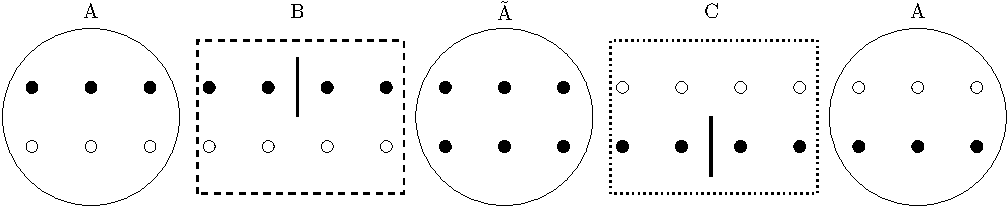
\includegraphics[scale = 0.8]{poglavlja/palindromi/slike/l_vecejednako_k-crop.pdf}
\caption{Primjer povezanosti elemenata dva presijecajuća palindroma (puni krugovi
	predstavljaju elemente palindroma) duljine $m=10$ za $2r \leq l$. Podebljane
	linije između elemenata predstavljaju sredine palindroma.}
\label{pal:fig:l_vecejednako_k}
\end{figure}

	\noindent
	Stoga, koristeći nezavisnost, funkciju $S$ i lemu \ref{pal:lem:mixvarijabli} dobivamo
	tvrdnju b).
%
\begin{multline*}
	\vP (\tsvar{Y}_i \cdot \tsvar{Y}_j =1 ) = 
	\prod_{t=m-1}^{l}
	\underbrace{
		\vP \left(
		\tsvar{X}_{i-t} =
		\ol{X}_{S(i-t, i-\frac{m}{2}+1, l)(1)} = 
		\tsvar{X}_{S(i-t, i-\frac{m}{2}+1, l)(2)} 
		\right)
	}_{\text{odnos A i \~A}}
	\cdot \\
	\prod_{t=k}^{l-1}
	\left[
		\underbrace{
		\vP \left(
		\tsvar{X}_{i-t} =
		\ol{X}_{S(i-t, i-\frac{m}{2}+1, l)(1)}
		\right)
		}_{B}
		\underbrace{
		\vP \left(
		\tsvar{X}_{j-t} =
		\ol{X}_{S(j-t, j-\frac{m}{2}+1, l)(1)}
		\right)
		}_{C}
	\right] = \\
		\prod_{v=i-m+1}^{i-l}
		\xi(v, i-\frac{m}{2}+1, l, 2) 
		\prod_{v=i-l+1}^{i-\frac{m}{2}}
		\xi(v, i-\frac{m}{2}+1, l, 1) 
		\prod_{v=j-l+1}^{j-\frac{m}{2}}
		\xi(v, j-\frac{m}{2}+1, l, 1) 
\end{multline*}

\noindent
	Slika \ref{pal:fig:2r_vece_l} prikazuje
	slučaj $2r>l$ i $l<\frac{m}{2}$. Budući da je $2r>l$ prvih $2r-l$ elemenata
	nalazi se u nizu $2q+3$ puta (uz komplementarnost na odgovarajućim
	mjestima), dok se ostalih $l-r$ elemenata na početku i na kraju
	nalazi u nizu $2q+1$ puta (uz komplementarnost na odgovarajućim
	mjestima).
	Stoga, koristeći nezavisnost, funkciju $S$ i lemu \ref{pal:lem:mixvarijabli} dobivamo
	tvrdnju d).
%
\begin{figure}[htb!]
\centering%
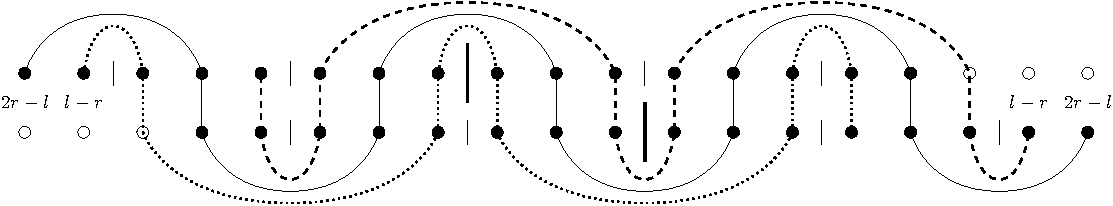
\includegraphics[scale = 0.8]{poglavlja/palindromi/slike/2r_vece_l-crop.pdf}
\caption{Primjer povezanosti elemenata dva presijecajuća palindroma (puni krugovi
	predstavljaju elemente palindroma) duljine $m=16$ za $2r>l$. Podebljane
	linije između elemenata predstavljaju sredine palindroma, a obične linije
	mjesta nužne simetrije.}
\label{pal:fig:2r_vece_l}
\end{figure}


	Ideja dokaza tvrdnje d) može se primjeniti i na tvrdnju c)
	pazeći da sada u početnom i krajnjem dijelu nemamo
	elemente koji se pojavljuju $2q+3$ puta.
\end{proof}

\begin{kor} \label{pal:kor:njdvjerojatnostpresjeka}
	Pretpostavimo da su $\tsvar{X}_n$ nezavisne jednako distribuirane slučajne
	varijable
	te neka je $l = j-i$. Označimo s $q$ i $r$ odgovarajuće
	koeficijente kod cjelobrojnog dijeljenja s ostatkom
	$\frac{m}{2} = q \cdot l + r$. Tada vrijedi
	\begin{itemize}
		\item[a)]{
			\text{za } $\frac{m}{2} \leq l \leq m-1$
			\[
				\vP( \tsvar{Y}_i \cdot \tsvar{Y}_j =1 ) =
				\left(
					\sum_{x \in \mathcal{A}} p_x^2 p_{\ol{x}} 
				\right)^{m-l}
				\left(
					\sum_{x \in \mathcal{A}} p_x p_{\ol{x}} 
				\right)^{2l-m}
			\]
		}
		\item[b)]{
			\text{za } $l < q$ i $2r \leq l$
			\[
				\vP( \tsvar{Y}_i \cdot \tsvar{Y}_j =1 ) =
				\left(
				\sum_{x \in \mathcal{A}} p_x^{q+1} p_{\ol{x}}^{q+1} 
				\right)^{2r}
				\left(
				\sum_{x \in \mathcal{A}} p_x^{q+1} p_{\ol{x}}^{q} 
				\right)^{l-2r}
			\]
		}
		\item[c)]{
			\text{za } $l < q$ i $2r > l$
			\[
				\vP( \tsvar{Y}_i \cdot \tsvar{Y}_j =1 ) =
				\left(
				\sum_{x \in \mathcal{A}} p_x^{q+1} p_{\ol{x}}^{q+1} 
				\right)^{2l-2r}
				\left(
				\sum_{x \in \mathcal{A}} p_x^{q+1} p_{\ol{x}}^{q+2} 
				\right)^{2r-l}
			\]
		}
	\end{itemize}
\end{kor}

\begin{proof}
Iz nezavisnosti i jednake distribuiranosti slučajnih varijabli
$X_n$, napomene \ref{pal:nap:njdmixvarijabli} te propozicije
\ref{pal:pro:opcavjerojatnostpresjeka} slijedi tvrdnja korolara.
\end{proof}

\noindent
Tvrdnju korolara \ref{pal:kor:njdvjerojatnostpresjeka}
kao i dokaz 
može se naći i u radu \textcite{leung_nonrandom_2005}. 

\begin{napomena_} \label{pal:nap:kovarijanca}
Koristeći lemu \ref{pal:lem:meanvarpalindroma} i propoziciju \ref{pal:pro:opcavjerojatnostpresjeka}
(jednakosti \ref{pal:eqn:meanpalindromanjd} i \ref{pal:eqn:varpalindromanjd} te korolar \ref{pal:kor:njdvjerojatnostpresjeka} u
n.j.d. slučaju) kovarijanca $\vCov{Y_i, Y_j}$ može se izračunati budući da vrijedi
\begin{gather}
	\vCov{\tsvar{Y}_i, \tsvar{Y}_j} =
	\vE{\tsvar{Y}_i \cdot \tsvar{Y}_j} - \vE{\tsvar{Y}_i} \vE{\tsvar{Y}_j}
	= \vP \left( \tsvar{Y}_i \cdot \tsvar{Y}_j  =1 \right)
	- \vP \left( \tsvar{Y}_i =1 \right) \vP \left( \tsvar{Y}_j  =1\right)
\end{gather}
\end{napomena_}

\begin{kor}
	Pretpostavimo da su $\tsvar{X}_n$ nezavisne jednako distribuirane slučajne
	varijable s uniformnom distribucijom nad abecedom $\mathcal{A}$.
	Tada su pojavljivanja palindroma na mjestu $i$ i mjestu $j$
	nezavisna za $i \neq j$. Odnosno, vrijedi jednakost
	\[
		\vP( \tsvar{Y}_i \cdot \tsvar{Y}_j =1 ) =  
		\vP( \tsvar{Y}_i=1) \vP( \tsvar{Y}_j=1) \ .
	\]
\end{kor}

\begin{proof}
	Ukoliko se palindromi ne sijeku	nezavisnost je očita.
	Ako se pak sijeku,
	za $\beta=\frac{1}{|\mathcal{A}|}$
	iz korolara \ref{pal:kor:njdvjerojatnostpresjeka} slijedi
	\begin{itemize}
		\item[a)]{
			\text{za } $\frac{m}{2} \leq l \leq m-1$
			\[
				\vP (\tsvar{Y}_i \cdot \tsvar{Y}_j =1 ) =
				\left(
					\sum_{x \in \mathcal{A}} \beta^2 \cdot \beta 
				\right)^{m-l}
				\left(
					\sum_{x \in \mathcal{A}} \beta \cdot \beta 
				\right)^{2l-m}
				=
				\left(
					\beta^2
				\right)^{m-l}
				\left(
					\beta
				\right)^{2l-m}
				=
				\beta^{m} \ ,
			\]
		}
		\item[b)]{
			\text{za } $l < q$ i $2r \leq l$
			\[
				\vP (\tsvar{Y}_i \cdot \tsvar{Y}_j =1 ) =
				\left(
				\sum_{x \in \mathcal{A}} \beta^{q+1} \beta^{q+1} 
				\right)^{2r}
				\left(
				\sum_{x \in \mathcal{A}} \beta^{q+1} \beta^{q} 
				\right)^{l-2r}
				=
				\left(
				\beta^{2q+1} 
				\right)^{2r}
				\left(
				\beta^{2q}
				\right)^{l-2r}
				=
				\beta^{m} \ ,
			\]
		}
		\item[c)]{
			\text{za } $l < q$ i $2r > l$
			\begin{multline*}	
				\vP (\tsvar{Y}_i \cdot \tsvar{Y}_j =1 ) =
				\left(
				\sum_{x \in \mathcal{A}} \beta^{q+1} \beta^{q+1} 
				\right)^{2l-2r}
				\left(
				\sum_{x \in \mathcal{A}} \beta^{q+1} \beta^{q+2} 
				\right)^{2r-l}
				\\
				=
				\left(
				\beta^{2q+1}
				\right)^{2l-2r}
				\left(
				\beta^{2q+2}
				\right)^{2r-l}
				=
				\beta^{m} \ .
			\end{multline*}
		}
	\end{itemize}
	%
	Nezavisnost sada slijedi iz 
	\ref{pal:pro:opcavjerojatnostpresjeka}
	budući da vrijedi
	\[
		\vP( \tsvar{Y}_i = 1) =
		\prod_{j=1}^{\frac{m}{2}} \left[
		\sum_{x \in \mathcal{A}}
		\beta \beta
		\right]
		=
		\beta^{\frac{m}{2}} \ , \quad
		\vP( \tsvar{Y}_i = 1) \vP(\tsvar{Y}_j = 1)
		= \beta^{2 \cdot \frac{m}{2}} = \beta^{m} \ .
	\]
\end{proof}

\section{Primjer primjene na stvarnim podacima}
\label{pal:sec:primjenanastvarnim}

Iako dublja analiza stvarnih DNA nizova u odnosu na broj palindroma
nije u području ovog doktorskog rada, svejedno će se u ovom potpoglavlju prezentirati
kratka analiza određenog DNA niza kao primjer primjene na stvarnim
podacima. 

Poznata je činjenica da frekvencije nukleobaza variraju
unutar DNA niza 
(\textcite{louie_nucleotide_2003} te \textcite{mrazek_strand_1998}).
Ovo je svojstvo
ilustrirano na slici \ref{pal:fig:AT_freq} za niz
{\glqq}Homo sapiens chromosome 1 genomic contig NT\_077912\_1''
\cite{ncbi_database_homosapiens}
duljine $153\, 649$.
Niz je podijeljen na blokove jednake duljine od
2000 znakova (parova) te su zbrojene frekvencije
komplementarnih baza $A$ i $T$.
Bitno je napomenuti da je duljina blokova odabrana proizvoljno
i ne mora nužno reprezentirati smislenu razdiobu na regije.
No, ukoliko se posjeduje ekspertno znanje o nizu nad kojim
se vrši istraživanje, blokove treba prilagoditi tom znanju.
Ekspertno je znanje od velike važnosti za analizu budući
da se kodirajuće i nekodirajuće regije uglavnom sastoje
od različitih distribucija baza 
(\textcite{roy_identification_2009}).

\begin{figure}
\centering
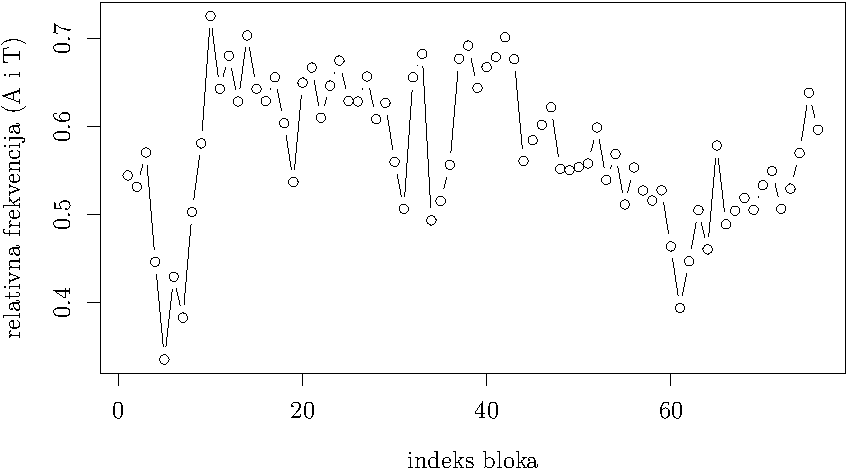
\includegraphics[scale = 1]{poglavlja/palindromi/slike/ATfreq_kromosom_1_blokovi_duljine_2000.pdf}
\caption{Zbrojene frekvencije od $A$ i $T$ po blokovima duljine 2000 za niz
{\glqq}Homo sapiens chromosome 1 genomic contig NT\_077912\_1''
\cite{ncbi_database_homosapiens}}
\label{pal:fig:AT_freq}
\end{figure}

\noindent  
Broj palindroma različitih duljina određen je po blokovima
te je rezultat o asimptotskoj normalnoj distribuciji
(pretpostavljajući da su blokovi tipa T1)
primijenjen pri izračunu vjerojatnosti dobivanja
broja palindroma minimalno velikog kao uočeni
($p$-vrijednosti ukoliko $\frac{N_n-\hat{\mu}_n}{\sqrt{n}}$
smatramo testnom statistikom). Rezultati za
palindrome duljina $6$ i $8$ prezentirani su u tablici
\ref{pal:tab:rezultatinahomosapiensu}. 

\begin{table}[htbp] 
\caption{Duljina niza $n=153\, 649$; za duljinu palindroma $m=6$
	bilo je 2464 palindroma dok je za duljinu palindroma $m=8$
	bilo 694 palindroma.}
\label{pal:tab:rezultatinahomosapiensu}
\centering
\begin{tabular}{ccccccc}
\hline
\multicolumn{1}{c}{} & \multicolumn{3}{c}{$m=6$} & \multicolumn{3}{c}{$m=8$} \\
\cmidrule(lr{0.75em}){2-4} \cmidrule(lr{0.75em}){5-7}
duljina blokova & $\frac{N_n-\hat{\mu}_n}{\sqrt{n}}$ & $\hat{\sigma}^2$ & p-vrijednost
& $\frac{N_n-\hat{\mu}_n}{\sqrt{n}}$ & $\hat{\sigma}^2$ & p-vrijednost \\
\hline
400 & -0.39555 & 0.01783 & 0.00153 & 0.0347 & 0.00458 & 0.3038\\ 
700 & -0.41628 & 0.017767 & 0.00089 & 0.0319 & 0.00456 & 0.3181\\ 
1000 & -0.42335  & 0.01772 & 0.00073 & 0.0322 & 0.00455 & 0.3162\\ 
1300 & -0.44870 & 0.01775 & 0.00037  & 0.0234 & 0.00457 & 0.3646\\ 
2000 & -0.45280 & 0.01770 & 0.00033  & 0.0236 & 0.00456 & 0.3633\\ 
n (n.j.d.) & -0.18075 & 0.01654 & 0.07995 & 0.12424  & 0.00422 & 0.02798\\ 
\hline 
\end{tabular} 
\end{table}

\noindent
Zanimljivo je primijetiti nepodudaranje modela s blokovima
s modelom u kojem pretpostavljamo nezavisnost i jednaku
distribuiranost. Za duljinu palindroma $m=6$ broj 
palindroma proglasili bi iznimnim, uz razinu značajnosti
od 5\%, za modele s blokovima dok istu vrijednost ne bi
proglasili iznimnom po n.j.d. modelu.
Obrnut slučaj možemo primijetiti kod palindroma duljine $m=8$
jer modeli s blokovima ne ukazuju na iznimnost za razliku od
n.j.d. modela.

Ovaj primjer tako pokazuje da bi korištenje n.j.d. modela moglo
dovesti do krivog tumačenja. Razlog leži u regijama s visokim
očekivanim brojem palindroma (zbog visokog postotka
komplementarnih baza) pa korištenjem n.j.d. modela
gubimo tu informaciju budući da usrednjavamo frekvencije.
Slobodno govoreći, model s blokovima je sposoban prepoznati
razlike među regijama dok n.j.d. model to isto nije sposoban
prepoznati. Stoga, n.j.d. model treba koristiti s oprezom.

Također, zanimljivo je primijetiti da se promjenom veličine
blokova p-vrijednosti ne mijenjaju znatno.




\appendix
\chapter{C++ k\^{o}d za optimalno poravnanje
Damerau-Levenshteinovim algoritmom}
\label{dodatak:levenshtein}

K\^{o}d prezentiran ovdje jest Proof-of-concept te
se zasniva na rekurzivnoj definiciji ne mareći
za efikasnost.

\begin{listing}{0}
#include <vector>
typedef std::vector<int> rijec;

rijec ptraj(int c, rijec t) {
    rijec nova;
    nova.push_back(c);
    nova.insert(nova.end(), t.begin(), t.end());
    return nova;
}

rijec ptraj(rijec c, rijec t) {
    c.insert(c.end(), t.begin(), t.end());
    return c;
}

struct levRez {
    int rez;
    std::vector<rijec> traj;

    levRez() {}
};

// MATCH=1, REPLACE=2, INSERT=3,
// DELETE=4, TRANSPOSITION=5
levRez damlev(rijec str1, rijec str2, int i, int j, rijec traj) {
    levRez lr;
    if (std::min(i, j) == 0) {
        if (i > 0)
            traj = ptraj(rijec(i, 4), traj);
        else if (j > 0)
            traj = ptraj(rijec(j, 3), traj);
        lr.rez = std::max(i, j);
        lr.traj.push_back(traj);
        return lr;
    }

    int x = 0;
    rijec tmp;
    if (str1[i - 1] !=
        str2[j - 1]) { // i-1 sluzi prilagodbi indeksiranju od nule
        x = 1;
        tmp = ptraj(2, traj);
    } else
        tmp = ptraj(1, traj);

    std::vector<levRez> L;
    L.push_back(damlev(str1, str2, i - 1, j, ptraj(4, traj)));
    L.push_back(damlev(str1, str2, i, j - 1, ptraj(3, traj)));
    L.push_back(damlev(str1, str2, i - 1, j - 1, tmp));

    int transp = 0;
    if (i > 2 && j > 2 && str1[i - 2] == str2[j - 1] &&
        str1[i - 1] == str2[j - 2]) {
        L.push_back(damlev(str1, str2, i - 2, j - 2, ptraj(5, traj)));
        transp = 1;
    }

    L[0].rez += 1;
    L[1].rez += 1;
    L[2].rez += x;
    int m = std::min(L[0].rez, L[1].rez);
    m = std::min(m, L[2].rez);
    lr.rez = m;

    if (transp) {
        L[3].rez += 1;
        lr.rez = std::min(lr.rez, L[3].rez);
    }

    // upisi minove u lr
    for (auto &x : L) {
        if (x.rez == lr.rez) {
            for (auto &y : x.traj) {
                lr.traj.push_back(y);
            }
        }
    }

    return lr;
}
\end{listing}

   
%%%%%%%%%%%%%%%%%%%%%%%%%%%%%%%%%%%%%%%%%%%%

\backmatter

\printbibliography[heading=bibintoc,
	notcategory=fullcited]

% za pojasnjenje naredbi \cleardoublepage i \phantomsection
% pogledati:
% https://tex.stackexchange.com/questions/57427/how-to-add-printindex-to-tableofcontents
% https://tex.stackexchange.com/questions/9191/when-do-i-need-invoke-clearpage-manually
% https://tex.stackexchange.com/questions/44088/when-do-i-need-to-invoke-phantomsection

\renewcommand{\glossarypreamble}{
	Popis odabranih stručnih pojmova s odgovarajućim
	engleskim prijevodom.}
\cleardoublepage
\phantomsection
\addcontentsline{toc}{chapter}{Kazalo pojmova}
\printglossary[title=Kazalo pojmova]

\cleardoublepage
\phantomsection
\renewcommand{\indexname}{Indeks pojmova}
\addcontentsline{toc}{chapter}{Indeks pojmova}
\printindex

\cleardoublepage
\phantomsection
\addcontentsline{toc}{chapter}{Popis slika}
\listoffigures

\chapter{Životopis}

Ivo Ugrina rođen je 21. svibnja 1983. godine u Splitu u Hrvatskoj.
U Splitu završava osnovnu i srednju školu te potom 2001. godine
upisuje Prirodoslovno-matematički fakultet u Zagrebu.
Za vrijeme studija obavlja dužnost demonstratora iz nekoliko
kolegija na inženjerskom smjeru matematike. U rujnu 2008. godine
uspješno brani diplomski rad  stekavši time titulu diplomiranog
inženjera matematike. Akademske godine 2008./2009. upisuje
doktorski studij matematike pri Prirodoslovno-matematičkom
fakultetu u Zagrebu gdje se i zapošljava kao asistent na 
projektu {\glqq}Mireo World'' u veljači 2009. godine.
Kao asistent u nastavi sudjelovao je u izvođenju vježbi iz
nekoliko računarskih i matematičkih kolegija. Tijekom
izobrazbe za doktora znanosti sudjelovao je u radu
seminara za Teoriju vjerojatnosti i matematičku statistiku.

Objavio je dva rada u SCIE referentnim časopisima te sudjelovao
na desetak konferencija, kako stručnih tako i znanstvenih.

\vspace{5ex}

\begin{center}
	\LARGE Bibliografija
\end{center}

\begin{easylist}[enumerate]
& \fullcite{spoljaric_statistical_2013}
& \fullcite{perkovic_multiparameter_2013}
\end{easylist}




%%%%%%%%%%%%%%%%%%%%%%%%%%%%%%%%%%%%%%%%%%%%

\end{document}
